\documentclass[12pt,letterpaper]{article}

\usepackage[T1]{fontenc}
\usepackage[margin=0.75in,headheight=1.5em]{geometry}
\usepackage{enumitem}
\usepackage{fancyhdr}
\usepackage{lastpage}
\usepackage{float}
\usepackage{tabu}
\usepackage{booktabs}
\usepackage{graphicx}
\usepackage{lmodern}
\usepackage[table]{xcolor}  
\usepackage[font=bf]{caption}

\begin{document}

\renewcommand\headrule{}

\pagestyle{fancy}
\fancyhf{}
\lfoot{COMP 3004}
\rfoot{\thepage/\pageref{LastPage}}
\cfoot{Requirements Analysis Document}

% CUSTOM COMMANDS
\newcommand{\twodigits}[1]{\ifnum\value{#1}<10 0\fi\arabic{#1}}

\newcommand{\teamname}{Code First, Think Later}
\newcommand{\personone}{Kevin Hua}
\newcommand{\persontwo}{Hendrik Knoetze}
\newcommand{\personthree}{Juhandr\'e Knoetze}

%% FIGURE COMMANDS
\newcommand{\figurelabel}[1]{\label{figure:#1}}
\newcommand{\figureref}[1]{\textbf{Figure \ref{figure:#1}}}
%% END FIGURE COMMANDS

%% TABLE COMMANDS
\definecolor{thcolor}{RGB}{193,193,193}
\newcommand{\ccindent}{\hspace{1.5em}\hangindent=1.5em}
\newcommand{\tableheader}{\rowfont\bf\rowcolor{thcolor!30}}

\newcommand{\tablelabel}[1]{\label{table:#1}}
\newcommand{\tableref}[1]{\textbf{Table \ref{table:#1}}}
%% END TABLE COMMANDS

%% USE-CASE COMMANDS
\newcounter{usecasenum}
\renewcommand{\theusecasenum}{\twodigits{usecasenum}}
\newcommand{\uclabel}[1]{\refstepcounter{usecasenum}\label{uc:#1}}
\newcommand{\ucref}[1]{\textbf{UC-\ref{uc:#1}}}
%% END USE-CASE COMMANDS

%% CLASS COMMANDS
\newcounter{classnum}
\renewcommand{\theclassnum}{\twodigits{classnum}}
\newcommand{\cllabel}[1]{\refstepcounter{classnum}\label{cl:#1}}
\newcommand{\clref}[1]{\textbf{CL-\ref{cl:#1}}}
%% END CLASS COMMANDS

%% STATE MACHINE COMMANDS
\newcounter{smnum}
\renewcommand{\thesmnum}{\twodigits{smnum}}
\newcommand{\smlabel}[1]{\refstepcounter{smnum}\label{sm:#1}}
\newcommand{\smref}[1]{SM-\ref{sm:#1}}
%% END STATE MACHINE COMMANDS

%% SEQUENCE DIAGRAM COMMANDS
\newcounter{seqnum}
\renewcommand{\theseqnum}{\twodigits{seqnum}}
\newcommand{\seqlabel}[1]{\refstepcounter{seqnum}\label{seq:#1}}
\newcommand{\seqref}[1]{SQ-\ref{seq:#1}}
%% END SEQUENCE DIAGRAM COMMANDS
% END CUSTOM COMMANDS

% TABLE STYLING
\everyrow{\hline}
\tabulinesep=0.5em

\setlist[itemize]{leftmargin=*,noitemsep,nolistsep}
\setlist[enumerate]{leftmargin=*,noitemsep,nolistsep}
% END TABLE STYLING

\thispagestyle{empty}

\begin{center}
	CARLETON UNIVERSITY
\end{center}

\vfill

\begin{center}
	{\fontsize{55pt}{55pt}\selectfont cuPID}
	\vspace{0.5em}\rule{\textwidth}{0.5pt}
	Requirements Analysis Document
\end{center}

\vspace{5em}

\begin{center}
	\textbf{Team [\teamname{}]}\\
	\personone{}\\
	\persontwo{}\\
	\personthree{}
\end{center}

\vfill

\begin{center}
	Submitted to:\\
	Dr. Christine Laurendeau\\
	COMP 3004: Object Oriented Software Engineering\\
	School of Computer Science\\
	Carleton University
\end{center}

\vspace{2em}

\begin{center}
	\today
\end{center}

\newpage{}

\tableofcontents{}

\renewcommand{\listfigurename}{Figures}
\listoffigures

\renewcommand{\listtablename}{Tables}
\listoftables

\newpage{}

\section{Introduction}

\begin{center}
    -- project --
\end{center}

\begin{center}
	\Huge [cuPID]
\end{center}

\begin{center}
    \rule{0.85\textwidth}{0.5pt}
\end{center}

\subsection{Purpose of System}

Team projects are typically assigned in University courses in order to develop and foster
good teamwork related skills, which are crucial in most future endeavours, notably 
prospective employment. Unfortunately, the task of separating students into balanced 
and compatible teams has always been a nigh impossible feat - hardly a year passes that doesn't
boast at least a single team brimming with  contention. There just seems to be too many
nuances that are involved in building a perfect team for professors to account for, often leading
to random or pseudo-random assignment of teams. Another possibility that professors might employ
would be to allow the students themselves to form their teams. Regrettably, this option also
leads to much strife - students tend to select friends or acquaintances as partners. While this
solution might seem good, it is sadly the case that good friends often make bad project partners. 
There is also the case that many students have not made friends or acquaintances yet that they 
could ask to be their partners, thus leaving them to form a team with others in their situation.

Both current options leave much to be desired. Our firm, [\teamname{}], has been hired
to design a system that would provide a better solution to this long-standing issue. Thus, the purpose of
our system is to separate students into teams with others of similar personality and skills, eliminating 
the frequent torment associated with ill-matched teams.

\subsection{Overview of Document}

This report provides an overview of the design decisions we made for the cuPID project, including 
use cases, object models, and dynamic models. The goal of this document is to clearly impart our vision of this
program to Dr. Christine Laurendeau, our esteemed client. In furtherance to this goal, we have painstakingly 
organized our report to maximize both basic legibility and traceability. Before delving into the more complex details 
of our proposed system, we have included a general overview of the elements we wish to incorporate, as well as 
some details with regards to our unique and innovative algorithm.

Following the short synopsis, you will find, the requested requirements, cleanly organized into separate functional 
and non-functional tables. Note that each requirement is assigned a unique but informative identifier - all future references
to this particular requirement will cite its corresponding code. The purpose of the system is, again, to ensure that the
reading of this document is as simple and pleasant an experience as possible. 

Directly after the requirements, we have the various system models. We have chosen to separate them into three
primary categories: the use cases, the objects, and the dynamic models. The goal of this separation scheme is to
stagger the introduction of different components such that the reader does not feel bombarded. Thus, you will 
first see the various possible scenarios and how the system will flow with regards to these scenarios. Subsequently, 
the various objects will be introduced and described in detail. Finally, we will delve into the more detailed sequence 
diagrams that will build on information from the prior sections. This section will handle such things as timings and
the flows for the various possible states of the system.

\vspace{1em}

\noindent Best regards,

\vspace{1em}

\begin{center}
	
\includegraphics[scale=0.4]{imgs/logo.png} \\ \footnotesize{(Team [Code First, Think Later])}
\end{center}

\vspace{1em}

\section{Proposed System}

\subsection{Overview}

The system that we are proposing to build offers a simplistic and clean interface designed for the single purpose of generating 
well-rounded and personality-compatible teams. To this end, we will allow two possible users: the Administrator, typically the professor,
and the Student. We want to really make a clear distinction between these two users - all that the Student user can do is access their
personal profile and control their participation to projects, while the Administration is in charge of all other aspects of project maintenance. 
Solely the Administrator will be able to run and view the results of our specialized Partner Matching Algorithm. This algorithm, broadly speaking,
will be analyzing four aspects of a person in order to generate the best possible teams:  programming or other relevant skills, leadership skills,
personality, and available. 

In this section, we will showcase a comprehensive breakdown of all the various components of our proposed system. For the sake of 
legibility, we have decided to organize the content in such a way that we move naturally from simplest to most complex - in other words,
each subsequent section builds off the previous. 

\subsection{Functional Requirements}

Functional requirements are the result of us carefully analzing the problem statement that you have submitted and extracting all the key 
desired features. In other words, we have converted your request into a list of requirements that we will fulfill. For example, you mention that
it is essential that this software can create projects. All the main features that you have expressed the desire to have have been matched with
the appropriate user and included in the following table, \tableref{fr}. 

\begin{table}[H]
	\caption{Functional Requirements}\tablelabel{fr}
	\begin{tabu} to \textwidth {>{\bf}l X}
	    \tableheader{}ID & Description\\
		F-01 & Students must be able to add themselves to any number of projects. \\
		F-02 & Students must be able to remove themselves from a project they are currently part of. \\
		F-03 & Students must be able to edit their Project Partner Profile. \\
		\ccindent{}F-03-01 & \ccindent{}Students must be able to modify the values representing their own qualifications. \\
		\ccindent{}F-03-02 & \ccindent{}Students must be able to modify the values representing what qualifications they
		desire in potential partners (what they prioritize, for example). \\
		F-04 & Students must be able to view their Project Partner Profile. \\
		F-05 & Administrators must be able to create new projects. \\
		F-06 & Administrators must be able to edit existing projects. \\
		\ccindent{}F-06-01 & \ccindent{}Administrators must be able to modify the team size parameter for individual projects. \\
		\ccindent{}F-06-02 & \ccindent{}Administrators must be able to add a student to a selected project. \\
		\ccindent{}F-06-03 & \ccindent{}Administrators must be able to remove a student from a selected project. \\
		\ccindent{}F-06-04 & \ccindent{}Administrators must be able to modify the project name parameter for individual projects.\\
		F-07 & Administrators must be able to launch the PPID for a specific project. \\
		F-08 & Administrators must be able to view the summary results of the last-run PPID. \\
		F-09 & Administrators must be able to view the detailed results of the last-run PPID. \\
	\end{tabu}
\end{table}

\subsection{Non-Functional Requirements}

Non-functional requirements are differentiable from the functional requirements in that they are not the requested features of the project, but
rather the various standards our proposed system must meet. For example, you expressed the desire that the system be designed specifically 
for use with the Linux Ubuntu platform, and that all code must be written in the C++ programming language. Also included in \tableref{nfr} are
assorted promises to meet various standards that you have not included in your problem statement but that either we believe should be required, 
or is required by law.

\begin{table}[H]
	\caption{Non-Functional Requirements}\tablelabel{nfr}
	\begin{tabu} to \textwidth {>{\bf}l >{\it}l X}
        % Categories left: Interface(2), Operation(1)
	    \tableheader{}ID & Category & Description\\
		NF-01 & Usability & The option to customize the key bindings for default keyboard short cuts must be available for all users.\\
		NF-02 & Usability & The option to change the interface colour scheme to accomodate for colour-blindness must be available for all users.\\
		NF-03 & Usability & The size of the 'buttons' on the interface must be large enough to accomodate for users that want to use a touch-screen monitor.\\
		NF-04 & Reliability & The system will not terminate due to errors 95\% of the time.\\
		NF-05 & Reliability & Saved data will remain uncorrupted at least 95\% of the time. \\
		NF-06 & Reliability & Saved information must be backed up. \\
		NF-07 & Implementation & The system must be written in the C++ language. \\
		NF-08 & Implementation & The system must use the Qt framework for creating the graphical user interface (G.U.I.). \\
		NF-09 & Implementation & The system must run in the Ubuntu 14.04 virtual machine. \\
		NF-10 & Performance & The PPID will take no longer than 5 seconds to finish running. \\
		NF-11 & Performance & The system will not take longer than 2 seconds to perform any save operation. \\
		NF-12 & Performance & The system will not take longer than 2 seconds to perform any load operation. \\
		NF-13 & Supportability & The system must be extensible to a client/server architecture. \\
		NF-14 & Supportability & The system must be portable to Windows and Mac operating systems. \\
		NF-15 & Supportability & Later system versions will support the saved data of at least the last two versions. \\
		NF-16 & Legal & Users must accept a Terms of Service agreement in order to use the software.\\
		NF-17 & Legal & The system will be released under the GPL (GNU General Public License). \\
		NF-18 & Legal & The software will not install any supplementary software onto the users computers without the users expressed consent (section 8 of CASL (Canada's Anti-Spam Legislation)).\\
	\end{tabu}
\end{table}

\begin{center}
\begin{tabu} to \textwidth {>{\bf}l >{\it}l X}
	\tableheader{} ID & Category & Description\\
		NF-19 & Interface & The software must provide an API to cuLearn.\\
		NF-20 & Interface & \\
		NF-21 & Interface & \\
		NF-22 & Operation & A forum should be provided for users to report any bugs they may encounter. \\
		NF-23 & Operation & There will be a call center available for any enquiries. \\
		NF-24 & Operation & \\
		NF-25 & Packaging & The software will be available to download as a standalone executable. \\
		NF-26 & Packaging & The client is in charge of installing it on their own machine. \\
		NF-27 & Packaging & Installation instructions will be included. \\
\end{tabu}
\end{center}

\subsection{System Models}

System models are some great tools that we have decided to incorporate into our system proposition to better convey the various functionalities and
interactions in our system. They provide a strong visual representation of the various ideas that we have, including general scenarios (use-cases) such as 
"Administrator creates a new project," interactions between different objects, and precise sequence diagrams that display what each object
does and for approximately how long. Specifically, you will be provided with use case diagrams with corresponding descriptions, entity, control, and boundary objects with corresponding  
dictionaries, state machine diagrams, and sequence diagrams. 

Use case diagrams and descriptions are useful for showcasing all the possible actions we want to incorporate into our system, with the added bonus of clearly
identifying the requirements each satisfies. Entity objects delve deeper and repesent all the users and other objects in the game, listing all the attributes and associations
that each has. The purpose of including this model is to exhibit all the potential behavior and aspects each object has access to. The next model, state machines, takes a large
step backwards; here we see a more abstracted view of the system - specifically, a diagram showing the possible states that each control object can experience. In other words, this
model does not see the system as a whole, but rather focuses on a very minute aspect of the system and explains how it works. Finally. sequence diagrams
expand on the previously mentioned use cases and transforms the detailed descriptions into visual representations that also display the proportion of time spent
at each step. Furthermore, the creation and destruction of objects is also displayed in this diagram. While it can be argued that each model exhibits varying levels
of informativeness, each is required to fully understand the next.

\subsubsection{Use Case Model}

Use case models are pairings of diagrams that depicts the actions that a specified user can take in a tree-like format with detailed descriptions of each action. The actions 
are divided into two three types: the high-level cases, denoted with <<initiates>>, the detailed cases, denoted with <<include>>, and the error cases, denoted with 
<<extend>>. To augment readability, we have decided to have a separate section for the high-level cases and grouping the detailed and error cases together. One 
concession we did make was to separate the different actions by {\it User}, or actor. 

The format of this section will be separated in two parts. For the first part, we will further subdivide into two parts: the high-level use cases and the detailed use cases. 
These two sub-sections will be identically formatted insofar as the diagrams will precede the more detailed descriptions, which are organized in a clean table format. Following
this first part, the second part will contain the more detailed flow of events for every use case in the previous part (both high-level and detailed).

\subsubsection*{High-level Use Cases}

This section contains the high-level use cases - essentially, the most abstracted action each user (actor) can take. The diagram below, \figureref{high-level-uc}, illustrates the interaction between
users, defined by the stick figure, and the system, defined by the rectangular box. The ovals represent the highest level actions that can be taken, with a connecting line to
the user that can initiate them. Specifically, we have the {\it Student User} who can initiate the high-level action of {\it ParticipateInProjects}, and we have the {\it Administrator User} 
who can initiate in the action of {\it ManageProject}. These actions are purposefully vague and general because they are the "parent action" that includes several other more specific actions.
\vspace{1em}

\begin{figure}[H]
	\centering{}
	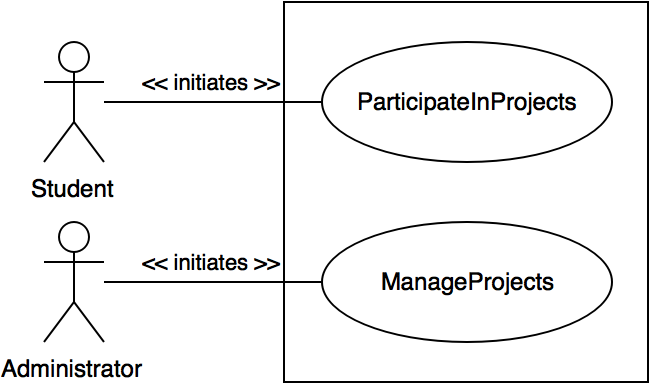
\includegraphics[scale=0.3]{imgs/high-level-use-case-diagram.png}
	\caption{High-level Use Case Diagram}\figurelabel{high-level-uc}
\end{figure}

Pulling the use cases from the diagram, we have next a list of the use cases in table format, \tableref{high-level-uc}, with a short and succinct descriptions beside. The purpose of this table,
on top of having the diagram, is for ease of access with regards to information. While it is very nice to see a diagram, nothing quite beats the traditional table when
it comes to laying out data. Another benefit is, like in the case of {\it EditProfile}, it shows what detailed use cases are included in these higher-level cases.

\begin{table}[H]
	\caption{High-Level Use Case Descriptions}\tablelabel{high-level-uc}
	\begin{tabu} to \textwidth {l >{\bf}l X}
	    \tableheader{}ID & Name & Description\\
	    \uclabel{manage-enrollment}\ucref{manage-enrollment} & ManageEnrollment & The Student accesses and modifies the projects the Student is enrolled in.\\
		\uclabel{edit-profile}\ucref{edit-profile} & EditProfile & The Student modifies the parameters of their profile (includes EditPersonalValues and EditDesiredValues).\\
		\uclabel{manage-project}\ucref{manage-project} & ManageProject & The Administrator manages projects as well as having the option to create a new instance of a project (includes manipulating student participation and access to the PPID and its results).\\
		\uclabel{create-new-project}\ucref{create-new-project} & CreateNewProject & The Administrator creates a new instance of a project.\\
	\end{tabu}
\end{table}

\subsubsection*{Detailed Use Cases}

This section contains the more detailed use cases - the specific cases, as it were, of the the much more general high-level use cases. Whereas the high-level cases help give a good
idea of how things are situated, detailed use cases are much more informative because they encompass all the finer details of the proposed software. Sure, it's nice to know that
an {\it Administrator} can {\it ManageProject}, but I am sure that you would agree with us that this is very vague. What exactly is "Managing Projects"? Well, that is the puprose of this 
section. 

The below figure and table, \figureref{detailed-admin-uc} and \tableref{detailed-uc-administrator}, cover the use cases that concern the {\it Administrator}.

\begin{figure}[H]
	\centering{}
	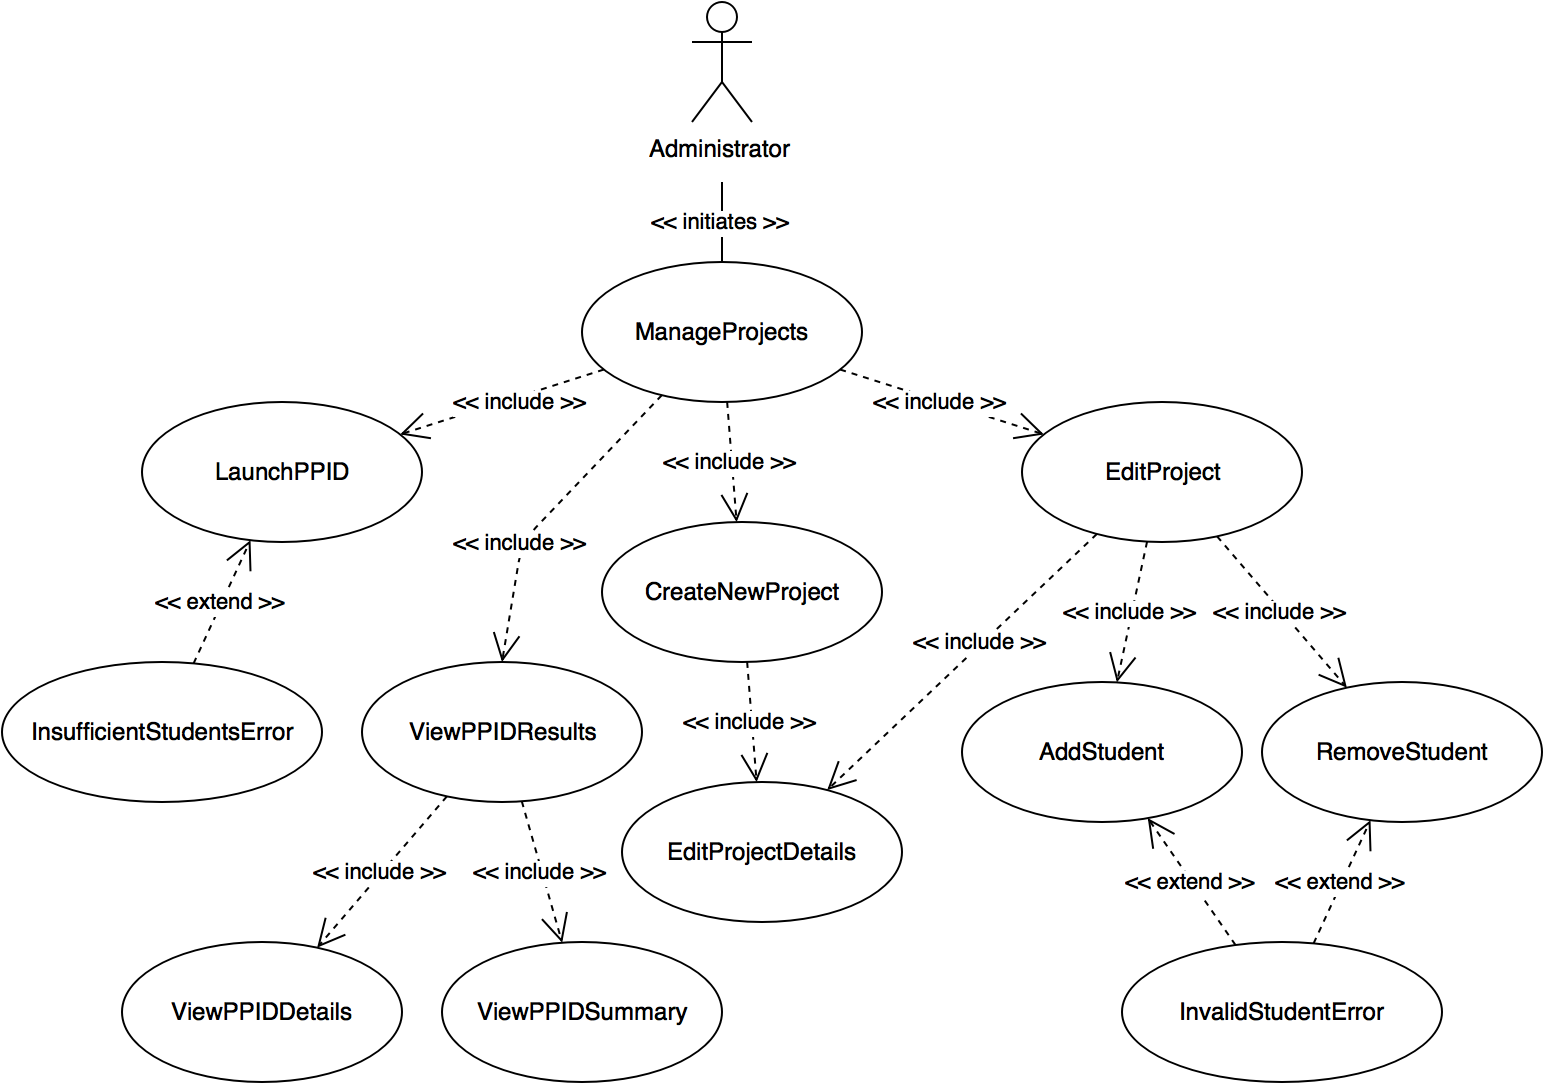
\includegraphics[scale=0.26]{imgs/detailed-administrator-use-case-diagram.png}
	\caption{Detailed Use Case Diagram - Administrator}
	\figurelabel{detailed-admin-uc}
\end{figure}
The next table, \tableref{detailed-uc-administrator} contains all the information about each particular use case for the {\it Administrator}, though forgoing the actual relationships. A unique identifier for each use case is also assignment here.. %CHANGE THIS PARAGRAPH

\begin{table}[H]
	\caption{Detailed Use Case Descriptions - Administrator}\tablelabel{detailed-uc-administrator}
	\begin{tabu} to \textwidth {l >{\bf}l X}
	    \tableheader{}ID & Name & Description\\
		\uclabel{launch-ppid}\ucref{launch-ppid} & LaunchPPID & The Administrator runs the PPID for a specified project.\\
		\uclabel{insufficient-students-error}\ucref{insufficient-students-error} & InsufficientStudentsError & The system reports that there are not enough Students registered in the project to run the PPID.\\
		\uclabel{view-ppid-results}\ucref{view-ppid-results} & ViewPPIDResults & The Administrator views the results of the PPID for a project.\\
		\uclabel{view-ppid-summary}\ucref{view-ppid-summary} & ViewPPIDSummary & The Administrator views a summary of the groups that are created.\\
		\uclabel{view-ppid-details}\ucref{view-ppid-details} & ViewPPIDDetails & The Administrator views a detailed analysis of the grouping decisions.\\
		\uclabel{edit-project-details}\ucref{edit-project-details} & EditProjectDetails & The Administrator modifies the parameters of a specified project.\\
		\uclabel{edit-project}\ucref{edit-project} & EditProject & The Administrator modifies an aspect of the project (includes Student participation and project parameters).\\
	\end{tabu}
\end{table}

The following figure, \figureref{detailed-student-uc}, outlines the use cases and their relationships with each other for the {\it Student User}. Note here that the {\it Student} has far fewer possible use cases
as compared to the {\it Administrator} - there are only two major things that {\it Students} can do: edit their profile, and manage their enrollment in projects. They have no 
access to finer details such as project settings. 

\begin{figure}[H]
	\centering{}
	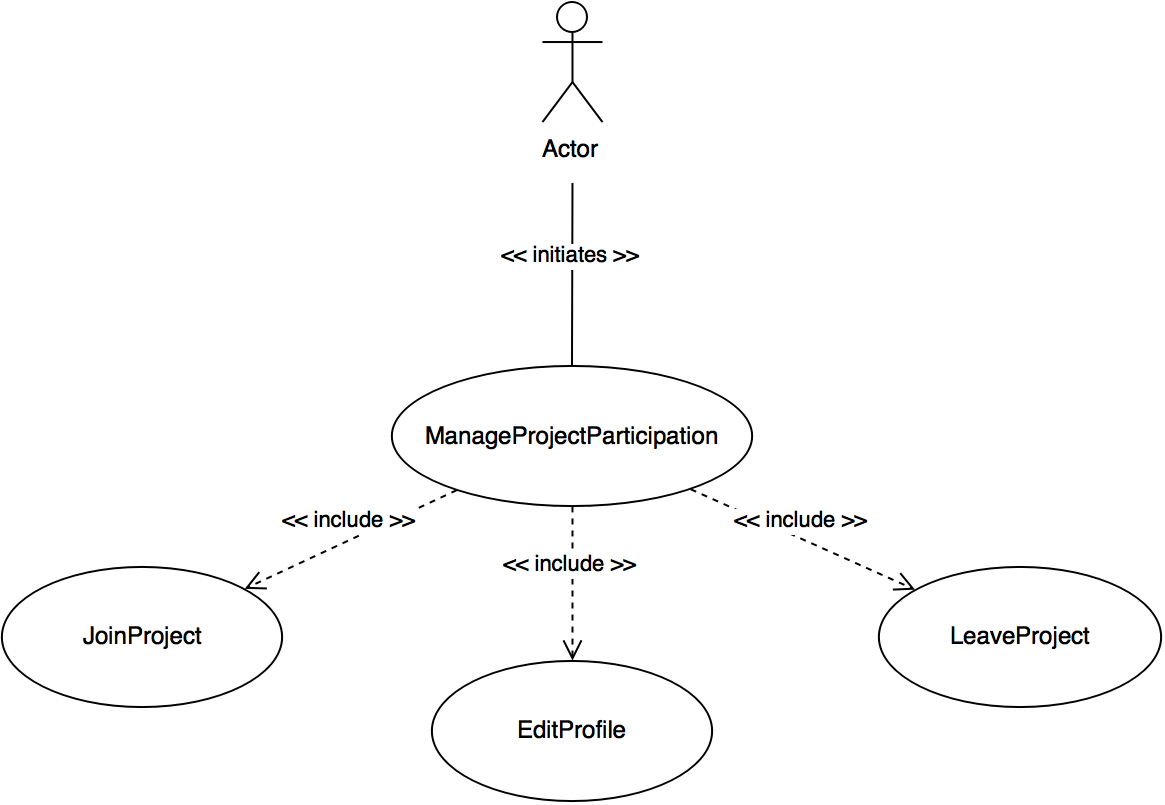
\includegraphics[scale=0.25]{imgs/detailed-student-use-case-diagram.png}
	\caption{Detailed Use Case Diagram - Student}
	\figurelabel{detailed-student-uc}
\end{figure}

\newpage{}

The ensuing table, \tableref{detailed-uc-student} describes each of the possible use cases that a {\it Student User} can use/encounter.
Please also note that we have decided to not include any error cases in this particular diagram to maximize legibility.

\begin{table}[H]
	\caption{Detailed Use Case Descriptions - Student}\tablelabel{detailed-uc-student}
	\begin{tabu} to \textwidth {l >{\bf}l X}
	    \tableheader{}ID & Name & Description\\
		\uclabel{join-project}\ucref{join-project} & JoinProject & The student adds themselves to an existing project.\\
		\uclabel{leave-project}\ucref{leave-project} & LeaveProject & The student removes themselves from an existing project.\\
		\uclabel{edit-personal-values}\ucref{edit-personal-values} & EditPersonalValues & The student modifies the personal details in his profile (what they have to offer).\\
		\uclabel{edit-desired-values}\ucref{edit-desired-values} & EditDesiredValues & The student modifies the desired details in his profile (what they are looking for in potential team members).\\
	\end{tabu}
\end{table}

The following diagram, \figureref{detailed-user-input-uc}, displays the possible ways each user can input into the system and their associated errors. Note that for most of the cases, the inputs are value-based and thus
all refer to the same {\it InvalidInputError} use case.

\begin{figure}[H]
	\centering{}
	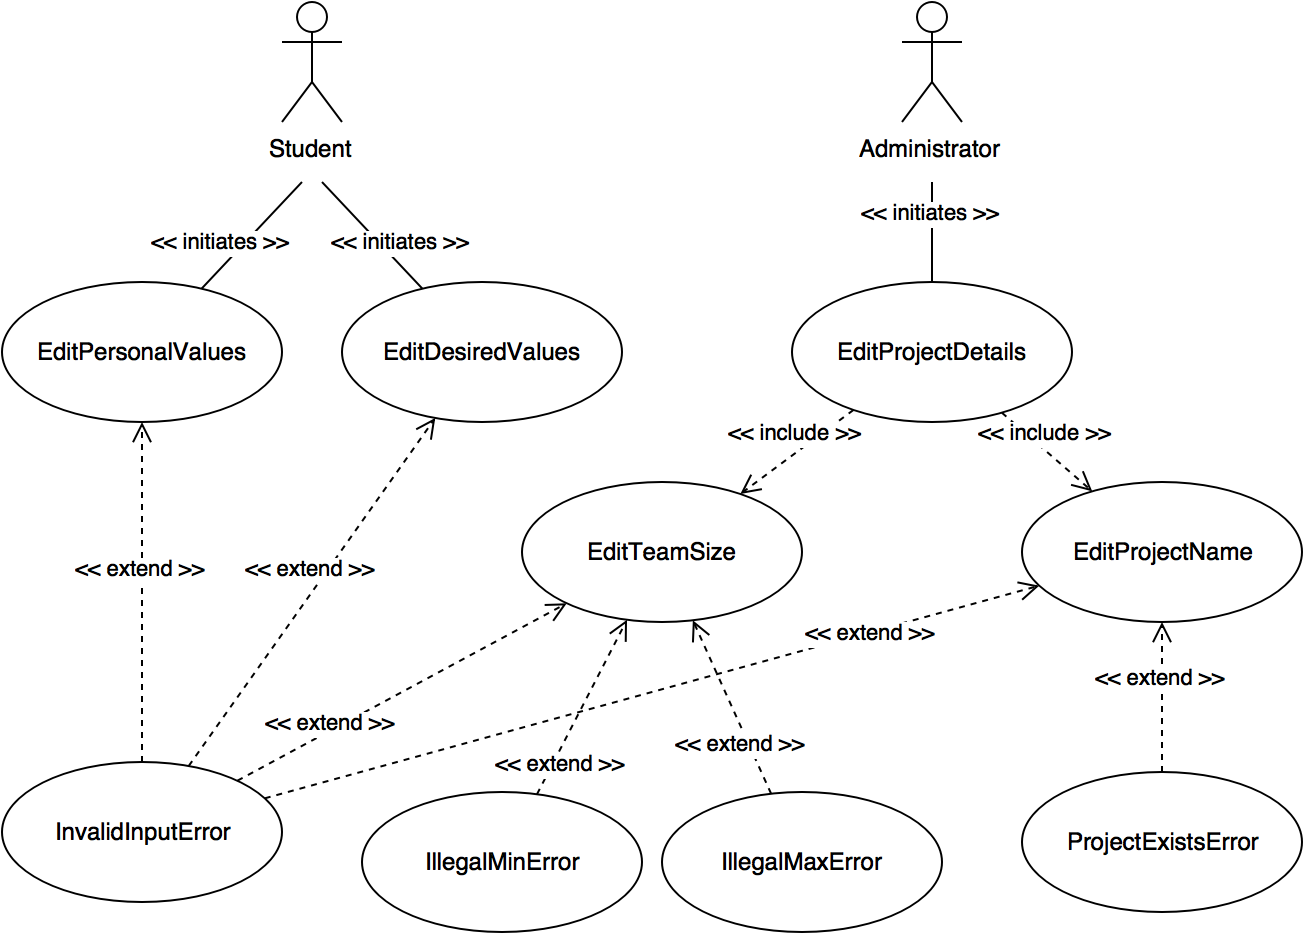
\includegraphics[scale=0.3]{imgs/detailed-user-input-use-case-diagram.png}
	\caption{Detailed Use Case Diagram - User Input}
	\figurelabel{detailed-user-input-uc}
\end{figure}

\tableref{detailed-uc-user-input}, the following table, pulls the use cases from \figureref{detailed-user-input-uc} and provides both a detailed description and a unique identifier for each. That said, please note that several of the cases present in \figureref{detailed-user-input-uc} are absent in this table - {\it EditPersonalValues}, {\it EditDesiredValues}, and {\it EditProjectDetails} all have already been described in \tableref{detailed-uc-administrator} and \tableref{detailed-uc-student}.

\begin{table}[H]
	\caption{Detailed Use Case Descriptions - User Input}\tablelabel{detailed-uc-user-input}
	\begin{tabu} to \textwidth {l >{\bf}l X}
	    \tableheader{}ID & Name & Description\\
		\uclabel{invalid-input-error}\ucref{invalid-input-error} & InvalidInputError & The system reports that the given value is invalid.\\
		\uclabel{edit-project-name}\ucref{edit-project-name} & EditProjectName & The Administrator sets the name of the project. \\
		\uclabel{project-exists-error}\ucref{project-exists-error} & ProjectExistsError & The system reports that a project with the given name already exists.\\
		\uclabel{edit-group-size}\ucref{edit-group-size} & EditGroupSize & The Administrator sets the minimum and maximum group sizes to be used by the PPID. \\
		\uclabel{invalid-group-size-error}\ucref{invalid-group-size-error} & InvalidGroupSizeError & The system reports that the given group size is illegal.\\
	\end{tabu}
\end{table}

The following diagram, \figureref{detailed-common-error-uc}, shows which use cases, for both the {\it Administrator} and the {\it Student} Users, can trigger the {\it StorageError} use case. In other words, which of the 
priorly mentioned use cases interact with reading files, writing files, and opening the Storage.

\begin{figure}[H]
	\centering{}
	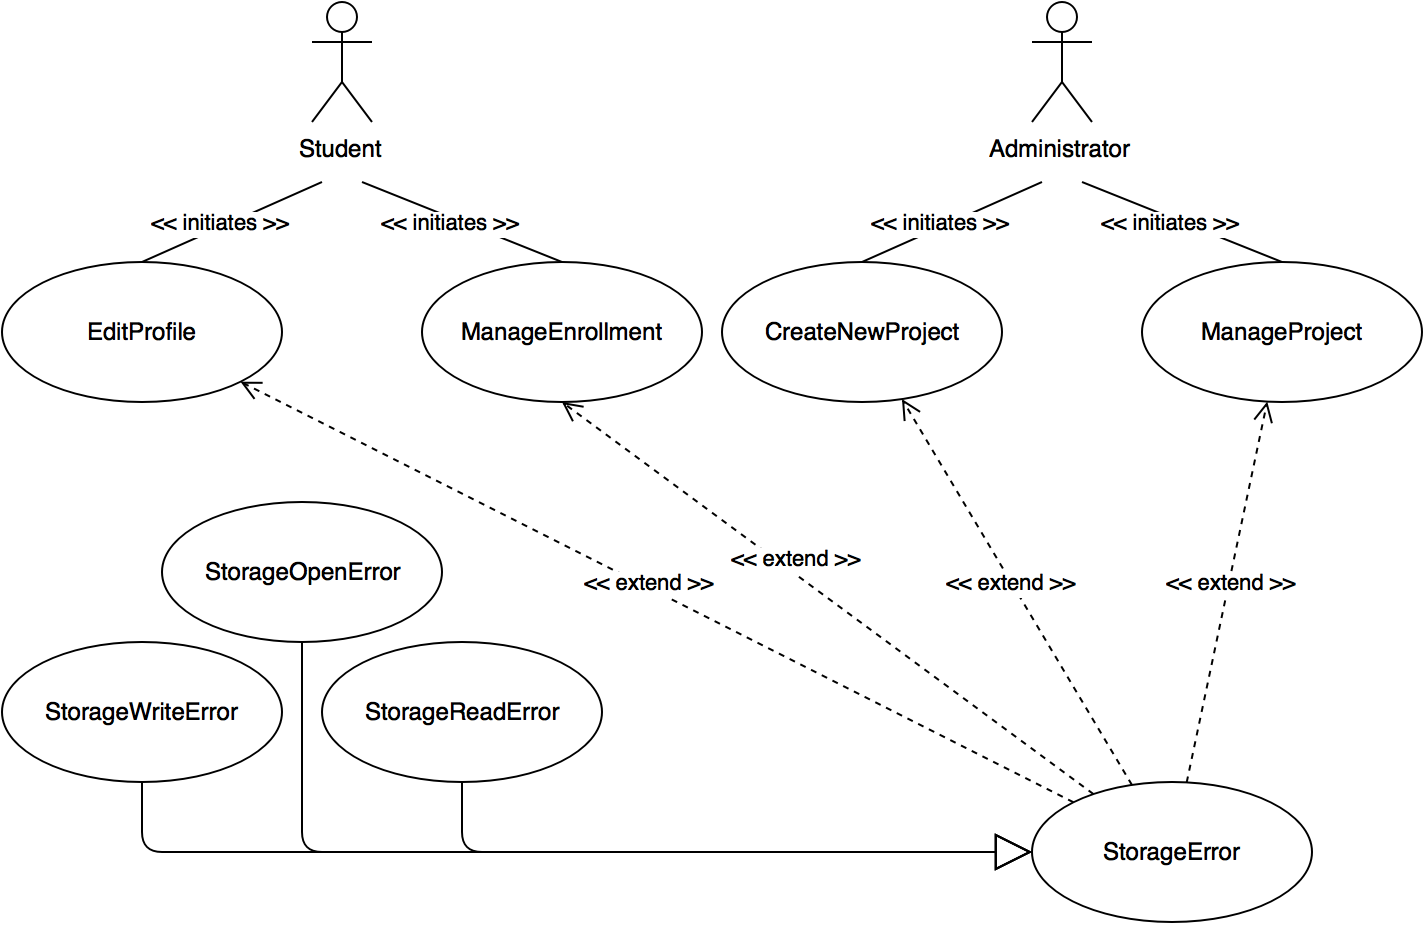
\includegraphics[scale=0.3]{imgs/detailed-common-error-use-case-diagram.png}
	\caption{Detailed Use Case Diagram - Common Errors}
	\figurelabel{detailed-common-error-uc}
\end{figure}

The table below, \tableref{detailed-uc-common-errors}, covers all the the descriptions and assignment of unique identifiers for the storage-related error use cases. Note that the first use case in this table, {\it StorageError}, is a generalization
of the other three use cases.

\begin{table}[H]
	\caption{Detailed Use Case Descriptions - Common Errors}\tablelabel{detailed-uc-common-errors}
	\begin{tabu} to \textwidth {l >{\bf}l X}
	    \tableheader{}ID & Name & Description\\
		\uclabel{storage-error}\ucref{storage-error} & StorageError &  The system reports that there is an error with the stored information for cuPID (generalizes StorageReadError, StorageOpenError, and StorageWriteError).\\
		\uclabel{storage-read-error}\ucref{storage-read-error} & StorageReadError & The system reports that an error occurred while attempting to read from the Storage.\\
		\uclabel{storage-open-error}\ucref{storage-open-error} & StorageOpenError & The system reports that an error occurred while attempting to open the Storage.\\
		\uclabel{storage-write-error}\ucref{storage-write-error} & StorageWriteError & The system reports that an error occurred while attempting to write to the Storage.\\
	\end{tabu}
\end{table}

\subsubsection*{Table-Based Use Case Flow of Events}

In the following section, we will delve into each of the priorly mentioned use cases in much more detail. Specifically, participating actors, detailed flow of events, entry/exit conditions, quality requirements, if applicable, and 
references to which requirements each address shall all be provided for each use case. To ensure ease of reading, we will maintain the exact same ordering as listed in the above section.

\vspace{1em}

The {\it ManageEnrollment} (\ucref{manage-enrollment}) allows Student actors to both join or leave existing projects. It is a high-level use case that includes both the {\it JoinProject} and the {\it LeaveProject} use cases.

\begin{center}
	\begin{tabu} to \textwidth {>{\it}l X}
		\toprule
		Use Case Identifier & \ucref{manage-enrollment} \\
		Name & {\bf ManageEnrollment} \\
		Participating Actors & Initiated by Student \\
		Flow of Events & 
		\begin{minipage}[t]{\linewidth}
		    \begin{enumerate}
			    \item[1.] The Student chooses the manage enrollment option.
			    \begin{enumerate}
			        \item[2.] The system displays a list of projects.
				\end{enumerate}
				\item[3.] The Student chooses a project.
				\begin{enumerate}
				    \item[4.] The system displays a menu with two options. The Student can choose to join the project (include use case \textbf{JoinProject}), or leave the project (include use case \textbf{LeaveProject}).
				\end{enumerate}
	        \end{enumerate}
		\end{minipage} \\

		Entry Conditions &
		\begin{minipage}[t]{\linewidth}
			\begin{itemize}
			    \item The User is operating cuPID as a Student.
	        \end{itemize}
		\end{minipage} \\

		Exit Conditions & \\


		Quality Requirements & \\

		Traceability & F-01, F-02\\
		\toprule
	\end{tabu}
\end{center}

\newpage{}

The {\it EditProfile} (\ucref{edit-profile}) allows Student actors to edit their profiles. Specifically, this is a high-level use case that includes both {\it EditPersonalValues} and {\it EditDesiredValues} use cases.

\begin{center}
	\begin{tabu} to \textwidth {>{\it}l X}
		\toprule
		Use Case Identifier & \ucref{edit-profile} \\
		Name & {\bf EditProfile} \\
		Participating Actors & Initiated by Student \\
		Flow of Events & 
		\begin{minipage}[t]{\linewidth}
		    \begin{enumerate}
		    		\item[1.] The Student chooses the edit profile option.
		    		\begin{enumerate}
			    		\item[2.] The system displays a menu with two options. The Student can choose to edit their own values for the attributes (include use case \textbf{EditPersonalValues}) or edit their desired partner values for the attributes (include use case \textbf{EditDesiredValues}).
		    		\end{enumerate}
			\end{enumerate}
		\end{minipage} \\

		Entry Conditions &
		\begin{minipage}[t]{\linewidth}
			\begin{itemize}
			    \item The User is operating cuPID as a Student.
	        \end{itemize}
		\end{minipage} \\

		Exit Conditions & \\

		Quality Requirements & \\

		Traceability &  F-03, F-03-01, F-03-02 \\
		\toprule
	\end{tabu}
\end{center}

\vspace{1em}
The {\it ManageProject} (\ucref{manage-project}) allows Administrator actors to manage project details. This is a high-level use case that
includes {\it LaunchPPID}, {\it ViewPPIDResults}, {\it EditProject}, and {\it DeleteProject}.

\begin{center}
  	  \begin{tabu} to \textwidth {>{\it}l X}
		\toprule
		Use Case Identifier & \ucref{manage-project} \\
		Name & {\bf ManageProject} \\
   	     Participating Actors & Initiated by Administrator \\
		Flow of Events & 
		\begin{minipage}[t]{\linewidth}
		    \begin{enumerate}
			    \item[1.] The Administrator selects the manage project option.
			    \begin{enumerate}
			        \item[2.] The system displays a list of projects.
				\end{enumerate}
				\item[3.] The Administrator chooses a project.
				\begin{enumerate}
				    \item[4.] The system displays a menu with three options. The Administrator can choose to launch the PPID (include use case \textbf{LaunchPPID}), view PPID results (include use case \textbf{ViewPPIDResults}), edit an existing project (include use case \textbf{EditProject}), or delete an existing project (include use case \textbf{DeleteProject}).
				\end{enumerate}
			\end{enumerate}
	    \end{minipage} \\

		Entry Conditions &
		\begin{minipage}[t]{\linewidth}
			\begin{itemize}
			    \item The User is operating cuPID as an Administrator.
	        \end{itemize}
	    \end{minipage} \\

		Exit Conditions & \\

		Quality Requirements & \\

		Traceability & F-05, F-06, F-07, F-08, F-09\\
        \toprule
    \end{tabu}
\end{center}

\newpage{}

The {\it CreateNewProject} (\ucref{create-new-project}) allows Administrator actors to create a new project. This is a high-level use case that includes the {\it EditProjectDetails} use case.

\begin{center}
	\begin{tabu} to \textwidth {>{\it}l X}
		\toprule
		Use Case Identifier & \ucref{create-new-project} \\
		Name & {\bf CreateNewProject} \\
		Participating Actors & Initiated by Administrator \\
		Flow of Events & 
		\begin{minipage}[t]{\linewidth}
		    \begin{enumerate}
			    \item[1.] The Administrator selects the create new project option.
			    \item[2.] The Administrator enters in the initial project values (include use case \textbf{EditProjectDetails}).
			    \begin{enumerate}
				    \item[3.] The system displays the new project to the Administrator.
				\end{enumerate}
		    \end{enumerate}
	    \end{minipage} \\

		Entry Conditions &
		\begin{minipage}[t]{\linewidth}
			\begin{itemize}
			    \item The User is operating cuPID as an Administrator.
			    \item The Administrator has chosen to create a new project.
	        \end{itemize}
	    \end{minipage} \\

		Exit Conditions & 
		\begin{minipage}[t]{\linewidth}
			\begin{itemize}
			    \item The project is created.
	        \end{itemize}
	    \end{minipage}\\

		Quality Requirements & \\

		Traceability & F-05 \\
		\toprule
	\end{tabu}
\end{center}

\vspace{1em}
The {\it LaunchPPID} (\ucref{launch-ppid}) allows Administrator actors to launch the sorting algorithm on a specified project and save the results.

\begin{center}
	\begin{tabu} to \textwidth {>{\it}l X}
		\toprule
		Use Case Identifier & \ucref{launch-ppid} \\
		Name & {\bf LaunchPPID} \\
		Participating Actors & Initiated by Administrator \\
		Flow of Events & 
		\begin{minipage}[t]{\linewidth}
		    \begin{enumerate}
			    \item[1.] The system computes the PPID results.
			    \item[2.] The system saves the PPID results.
			    \item[3.] The system notifies the Administrator that the results have been computed.
			\end{enumerate}
	    \end{minipage} \\

		Entry Conditions &
		\begin{minipage}[t]{\linewidth}
			\begin{itemize}
			    \item The User is operating cuPID as an Administrator.
			    \item The Administrator has chosen to run the PPID.
	        \end{itemize}
	    \end{minipage} \\

		Exit Conditions &
		\begin{minipage}[t]{\linewidth}
			\begin{itemize}
			    \item The PPID results are saved.
			    \item The PPID results are displayed to the Administrator.
	        \end{itemize}
	    \end{minipage} \\

		Quality Requirements &
		\begin{minipage}[t]{\linewidth}
			\begin{itemize}
			    \item The PPID will take no longer than 5 seconds to complete.
	        \end{itemize}
	    \end{minipage} \\

		Traceability & F-07, NF-05 \\
		\toprule
	\end{tabu}
\end{center}

\newpage{}

The {\it InsufficientStudentsError} (\ucref{insufficient-students-error}) allows the system to notify the Administrator actor if the Administrator actor attempts to run the PPID when there are
insufficient students in the project.

\begin{center}
	\begin{tabu} to \textwidth {>{\it}l X}
		\toprule
		Use Case Identifier & \ucref{insufficient-students-error} \\
		Name & {\bf InsufficientStudentsError} \\
		Participating Actors & Communicates with Administrator \\
		Flow of Events & 
		\begin{minipage}[t]{\linewidth}
		    \begin{enumerate}
			    \item[1.] The system informs the Administrator that there isn't enough Students in the Project to launch the PPID.
			    \item[2.] The launch of the PPID is stopped.
			\end{enumerate}
	    \end{minipage} \\

		Entry Conditions &
		\begin{minipage}[t]{\linewidth}
			\begin{itemize}
			    \item This use case \textbf{extends} the LaunchPPID use case. It is initiated by the Administrator whenever the Administrator launches the PPID on a project but there are not enough students to satisfy the minimum group size.
	        \end{itemize}
	    \end{minipage} \\

		Exit Conditions &
		\begin{minipage}[t]{\linewidth}
			\begin{itemize}
			    \item The launch of the PPID is stopped.
	        \end{itemize}
	    \end{minipage} \\

		Quality Requirements & \\

		Traceability & NF-04 \\
		\toprule
	\end{tabu}
\end{center}

\vspace{1em}
The {\it ViewPPIDResults} (\ucref{view-ppid-results}) allows the Administrator actor to view the results of the last run PPID for the specified project. Includes the {\it ViewPPIDSummary} and {\it ViewPPIDDetails} cases.

\begin{center}
	\begin{tabu} to \textwidth {>{\it}l X}
		\toprule
		Use Case Identifier & \ucref{view-ppid-results} \\
		Name & {\bf ViewPPIDResults} \\
		Participating Actors & Initiated by Administrator \\
		Flow of Events & 
		\begin{minipage}[t]{\linewidth}
		    \begin{enumerate}
		        \item[1.] The system displays a menu with two options. The Administrator can choose to view summary PPID results (include use case \textbf{ViewPPIDSummary}) or view detailed PPID results (include use case \textbf{ViewPPIDDetails}).
			\end{enumerate}
	    \end{minipage} \\

		Entry Conditions &
		\begin{minipage}[t]{\linewidth}
			\begin{itemize}
			    \item The User is operating cuPID as an Administrator.
			    \item The Administrator has chosen to view the PPID results, or the Administrator has finished launching the PPID.
	        \end{itemize}
	    \end{minipage} \\

		Exit Conditions & \\

		Quality Requirements & \\

		Traceability & F-08, F-09 \\
		\toprule
	\end{tabu}
\end{center}

\newpage{}

The {\it ViewPPIDSummary} (\ucref{view-ppid-summary}) allows Administrator actors to see the print out of the final decision of the PPID. In other words, it allows the Administrator to see the different groups that the PPID came up with.

\begin{center}
	\begin{tabu} to \textwidth {>{\it}l X}
		\toprule
		Use Case Identifier & \ucref{view-ppid-summary} \\
		Name & {\bf ViewPPIDSummary} \\
		Participating Actors & Initiated by Administrator \\
		Flow of Events & 
		\begin{minipage}[t]{\linewidth}
		    \begin{enumerate}
		        \item[1.] The system displays a print out of each group, including the students in each group.
			\end{enumerate}
	    \end{minipage} \\

		Entry Conditions &
		\begin{minipage}[t]{\linewidth}
			\begin{itemize}
			    \item The User is operating cuPID as an Administrator.
			    \item The Administrator has chosen to view the PPID summary.
	        \end{itemize}
	    \end{minipage} \\

		Exit Conditions & \\

		Quality Requirements & \\

		Traceability & F-08 \\
		\toprule
	\end{tabu}
\end{center}

\vspace{1em}
The {\it ViewPPIDDetails} (\ucref{view-ppid-details}) allows Administrator actors to see the actual steps and reasoning of the PPID with regards to the last run PPID. This print out does include the decision (actual groups it decided on) as well
as the inner-details.

\begin{center}
	\begin{tabu} to \textwidth {>{\it}l X}
		\toprule
		Use Case Identifier & \ucref{view-ppid-details} \\
		Name & {\bf ViewPPIDDetails} \\
		Participating Actors & Initiated by Administrator \\
		Flow of Events & 
		\begin{minipage}[t]{\linewidth}
		    \begin{enumerate}
		        \item[1.] The system displays the reasoning behind the computed groupings.
			\end{enumerate}
	    \end{minipage} \\

		Entry Conditions &
		\begin{minipage}[t]{\linewidth}
			\begin{itemize}
			    \item The User is operating cuPID as an Administrator.
			    \item The Administrator has chosen to view the PPID grouping details.
	        \end{itemize}
	    \end{minipage} \\

		Exit Conditions & \\

		Quality Requirements & \\

		Traceability & F-09 \\
		\toprule
	\end{tabu}
\end{center}

\newpage{}

The {\it EditProjectDetails} (\ucref{edit-project-details}) allows Administrator actors to modify project details like the possible group sizes and project name. Includes the {\it EditGroupSize} and {\it EditProjectName} use cases.

\begin{center}
	\begin{tabu} to \textwidth {>{\it}l X}
		\toprule
		Use Case Identifier & \ucref{edit-project-details} \\
		Name & {\bf EditProjectDetails} \\
		Participating Actors & Initiated by Administrator \\
		Flow of Events & 
		\begin{minipage}[t]{\linewidth}
		    \begin{enumerate}
			    \item[1.] The system displays a menu with two options. The Administrator can choose to edit the minimum and maximum group size (include use case \textbf{EditGroupSize}), or the name of the Project (include use case \textbf{EditProjectName}).
			    \item[2.] The system saves the project details.
			\end{enumerate}
		\end{minipage} \\

		Entry Conditions &
		\begin{minipage}[t]{\linewidth}
			\begin{itemize}
			    \item The User is operating cuPID as an Administrator.
			    \item The Administrator has chosen to edit existing, or set the initial, project details.
	        \end{itemize}
		\end{minipage} \\

		Exit Conditions &
		\begin{minipage}[t]{\linewidth}
			\begin{itemize}
			    \item The project details have been saved.
	        \end{itemize}
		\end{minipage} \\


		Quality Requirements & \\

		Traceability & F-05, F-06, F-06-01, F-06-04 \\
		\toprule
	\end{tabu}
\end{center}

\vspace{1em}
The {\it EditProject} (\ucref{edit-project}) allows Administrator actors to edit project details. Includes the {\it EditProjectDetails} use case.

\begin{center}
	\begin{tabu} to \textwidth {>{\it}l X}
		\toprule
		Use Case Identifier & \ucref{edit-project} \\
		Name & {\bf EditProject} \\
		Participating Actors & Initiated by Administrator \\
		Flow of Events & 
		\begin{minipage}[t]{\linewidth}
		    \begin{enumerate}
		        \item[1.] The Administrator enters in new project values (include use case \textbf{EditProjectDetails}).
			    \begin{enumerate}
			        \item[2.] The system displays the updated project to the Administrator.
			    \end{enumerate}
			\end{enumerate}
		\end{minipage} \\

		Entry Conditions &
		\begin{minipage}[t]{\linewidth}
			\begin{itemize}
			    \item The Administrator has chosen to edit a Project.
	        \end{itemize}
		\end{minipage} \\

		Exit Conditions &
        \begin{minipage}[t]{\linewidth}
			\begin{itemize}
			    \item The project is updated.
	        \end{itemize}
		\end{minipage} \\

		Quality Requirements & \\

		Traceability & F-06 \\
		\toprule
	\end{tabu}
\end{center}

\newpage{}

The {\it JoinProject} (\ucref{join-project}) allows Student actors to add themselves to an existing project that they are not already part of.

\begin{center}
	\begin{tabu} to \textwidth {>{\it}l X}
		\toprule
		Use Case Identifier & \ucref{join-project} \\
		Name & {\bf JoinProject} \\
		Participating Actors & Initiated by Student \\
		Flow of Events & 
		\begin{minipage}[t]{\linewidth}
		    \begin{enumerate}
				\item[1.] The system adds the Student to the selected project.
				\item[2.] The system notifies the Student that they have been added to the project.
			\end{enumerate}
		\end{minipage} \\

		Entry Conditions &
		\begin{minipage}[t]{\linewidth}
			\begin{itemize}
			    \item The User is operating cuPID as a Student.
			    \item The Student has selected to join a project.
	        \end{itemize}
		\end{minipage} \\

		Exit Conditions &
		\begin{minipage}[t]{\linewidth}
			\begin{itemize}
			    \item The addition of the Student to a project has been saved.
	        \end{itemize}
		\end{minipage} \\

		Quality Requirements & \\

		Traceability & F-01 \\
		\toprule
	\end{tabu}
\end{center}

\vspace{1em}
The {\it LeaveProject} (\ucref{leave-project}) allows Students actors to remove themselves from an existing project that they are a part of.

\begin{center}
	\begin{tabu} to \textwidth {>{\it}l X}
		\toprule
		Use Case Identifier & \ucref{leave-project} \\
		Name & {\bf LeaveProject} \\
		Participating Actors & Initiated by Student \\
		Flow of Events & 
		\begin{minipage}[t]{\linewidth}
		    \begin{enumerate}
			    \item[1.] The Student selects a project from a list of their joined projects.
			    \begin{enumerate}
			    		\item[2.] The system removes the Student from the selected project.
					\item[3.] The system notifies the Student that they have been removed from the project.
			    \end{enumerate}
			\end{enumerate}
		\end{minipage} \\

		Entry Conditions &
		\begin{minipage}[t]{\linewidth}
			\begin{itemize}
			    \item The User is operating cuPID as a Student.
			    \item The Student has chosen to remove themselves from a project.
	        \end{itemize}
		\end{minipage} \\

		Exit Conditions &
		\begin{minipage}[t]{\linewidth}
			\begin{itemize}
			    \item The removal of the Student from a project has been saved.
	        \end{itemize}
		\end{minipage} \\

		Quality Requirements & \\

		Traceability & F-02 \\
		\toprule
	\end{tabu}
\end{center}

\newpage{}

The {\it EditPersonalValues} (\ucref{edit-personal-values}) allows Students to modify the values for the section pertaining to their personal details.

\begin{center}
	\begin{tabu} to \textwidth {>{\it}l X}
		\toprule
		Use Case Identifier & \ucref{edit-personal-values} \\
		Name & {\bf EditPersonalValues} \\
		Participating Actors & Initiated by Student \\
		Flow of Events & 
		\begin{minipage}[t]{\linewidth}
		    \begin{enumerate}
		        \item[]
		        \begin{enumerate}
				    \item[1.] The system displays a menu of the Student's personal values that they can edit.
		        \end{enumerate}
	            \item[2.] The Student edits their personal values.
	            \begin{enumerate}
				    \item[3.] The system saves the Student's personal values.
		        \end{enumerate}
			\end{enumerate}
		\end{minipage} \\

		Entry Conditions &
		\begin{minipage}[t]{\linewidth}
			\begin{itemize}
			    \item The User is operating cuPID as a Student.
			    \item The Student has chosen to edit their personal values.
	        \end{itemize}
		\end{minipage} \\

		Exit Conditions &
		\begin{minipage}[t]{\linewidth}
			\begin{itemize}
			    \item The updated personal values have been saved.
	        \end{itemize}
		\end{minipage} \\

		Quality Requirements & \\

		Traceability &  F-03-01\\
		\toprule
	\end{tabu}
\end{center}

\vspace{1em}
The {\it EditDesiredValues} (\ucref{edit-desired-values}) allows Student actors to modify the values for the section pertaining to the values they desire in teammates.

\begin{center}
	\begin{tabu} to \textwidth {>{\it}l X}
		\toprule
		Use Case Identifier & \ucref{edit-desired-values} \\
		Name & {\bf EditDesiredValues} \\
		Participating Actors & Initiated by Student \\
		Flow of Events & 
		\begin{minipage}[t]{\linewidth}
		    \begin{enumerate}
		        \item[]
		        \begin{enumerate}
				    \item[1.] The system displays a menu of the Student's desired values that they can edit.
		        \end{enumerate}
	            \item[2.] The Student edits their desired values.
	            \begin{enumerate}
				    \item[3.] The system saves the Student's desired values.
		        \end{enumerate}
			\end{enumerate}		
		\end{minipage} \\

		Entry Conditions &
		\begin{minipage}[t]{\linewidth}
			\begin{itemize}
			    \item The User is operating cuPID as a Student.
			    \item The Student has chosen to edit their desired values.
	        \end{itemize}
		\end{minipage} \\

		Exit Conditions &
		\begin{minipage}[t]{\linewidth}
			\begin{itemize}
			    \item The updated desired values have been saved.
	        \end{itemize}
		\end{minipage} \\

		Quality Requirements & \\

		Traceability &  F-03-02\\
		\toprule
	\end{tabu}
\end{center}

\newpage{}

The {\it InvalidInputError} (\ucref{invalid-input-error}) allows the system to notify the Administrator or Student actors when they input incorrect values.

\begin{center}
	\begin{tabu} to \textwidth {>{\it}l X}
		\toprule
		Use Case Identifier & \ucref{invalid-input-error} \\
		Name & {\bf InvalidInputError} \\
		Participating Actors & Communicates with Administrator, Student \\
		Flow of Events & 
		\begin{minipage}[t]{\linewidth}
		    \begin{enumerate}
			    \item[1.] The system informs the Administrator/Student that the entered input is invalid.
			    \item[2.] Reverts the input to its original value.
		  \end{enumerate}
		\end{minipage} \\

		Entry Conditions &
		\begin{minipage}[t]{\linewidth}
			\begin{itemize}
			    \item This use case \textbf{extends} EditPersonalValues, EditDesiredValues, EditProjectName, and EditGroupSize. This is initiated by the Administrator/Student when the Administrator/Student inputs invalid data. 
	        \end{itemize}
		\end{minipage} \\

		Exit Conditions &
		\begin{minipage}[t]{\linewidth}
			\begin{itemize}
			    \item The invalid input is removed, and the input is reverted to its original value.
	        \end{itemize}
		\end{minipage} \\

		Quality Requirements & \\

		Traceability & NF-04 \\
		\toprule
	\end{tabu}
\end{center}

\vspace{1em}
The {\it EditProjectName} (\ucref{edit-project-name}) allows Administrator actors to modify the name of the current project.

\begin{center}
	\begin{tabu} to \textwidth {>{\it}l X}
		\toprule
		Use Case Identifier & \ucref{edit-project-name} \\
		Name & {\bf EditProjectName} \\
		Participating Actors & Initiated by Administrator \\
		Flow of Events & 
		\begin{minipage}[t]{\linewidth}
		    \begin{enumerate}
			    \item[1.] The Administrator inputs a unique project name.
			    \begin{enumerate}
			        \item[2.] The system updates the project name.
			        \item[3.] The system notifies the Administrator that the name has updated.
			    \end{enumerate}
			\end{enumerate}
		\end{minipage} \\

		Entry Conditions &
		\begin{minipage}[t]{\linewidth}
			\begin{itemize}
			    \item The User is operating cuPID as an Administrator.
			    \item The Administrator has chosen to set the project name.
	        \end{itemize}
		\end{minipage} \\

		Exit Conditions &
		\begin{minipage}[t]{\linewidth}
			\begin{itemize}
			    \item The project name is updated.
	        \end{itemize}
		\end{minipage} \\

		Quality Requirements & \\

		Traceability & F-06-04 \\
		\toprule
	\end{tabu}
\end{center}

\newpage{}

The {\it ProjectExistsError} (\ucref{project-exists-error}) allows the system to notify the Administrator actor if the desired project name is already in use.

\begin{center}
	\begin{tabu} to \textwidth {>{\it}l X}
		\toprule
		Use Case Identifier & \ucref{project-exists-error} \\
		Name & {\bf ProjectExistsError} \\
		Participating Actors & Communicates with Administrator \\
		Flow of Events & 
		\begin{minipage}[t]{\linewidth}
		    \begin{enumerate}
			    \item[1.] The system informs the Administrator that the project name is already in use.
			    \item[2.] The saving of an updated project is cancelled.
			\end{enumerate}
		\end{minipage} \\

		Entry Conditions &
		\begin{minipage}[t]{\linewidth}
			\begin{itemize}
			    \item This \textbf{extends} the EditProjectDetails use case. It is initiated by the Administrator when the attempts to save a project that has the same project name as an existing project.
	        \end{itemize}
		\end{minipage} \\

		Exit Conditions &
		\begin{minipage}[t]{\linewidth}
			\begin{itemize}
			    \item The project update is cancelled and the project name is reverted to its original value.
	        \end{itemize}
		\end{minipage} \\

		Quality Requirements & \\

		Traceability & NF-04 \\
		\toprule
	\end{tabu}
\end{center}

\vspace{1em}
The {\it EditGroupSize} (\ucref{edit-group-size}) allows Administrator actors to modify the range of possible group sizes, which includes the maximum and minimum values.

\begin{center}
	\begin{tabu} to \textwidth {>{\it}l X}
		\toprule
		Use Case Identifier & \ucref{edit-group-size} \\
		Name & {\bf EditGroupSize} \\
		Participating Actors & Initiated by Administrator \\
		Flow of Events & 
		\begin{minipage}[t]{\linewidth}
		    \begin{enumerate}
			    \item[1.] The Administrator inputs a new value for the minimum or maximum group size.
			    \begin{enumerate}
			        \item[2.] The system updates the project's minimum and maximum group size values.
			        \item[3.] The system notifies the Administrator that the group size has updated.
			    \end{enumerate}
			\end{enumerate}
		\end{minipage} \\

		Entry Conditions &
		\begin{minipage}[t]{\linewidth}
			\begin{itemize}
			    \item The User is operating cuPID as an Administrator.
			    \item The Administrator has chosen to update the group size.
	        \end{itemize}
		\end{minipage} \\

		Exit Conditions &
		\begin{minipage}[t]{\linewidth}
			\begin{itemize}
			    \item The group size is updated.
	        \end{itemize}
		\end{minipage} \\

		Quality Requirements & \\

		Traceability & F-06-01 \\
		\toprule
	\end{tabu}
\end{center}

\newpage{}

The {\it InvalidGroupSizeError} (\ucref{invalid-group-size-error}) allows the system to notify the Administrator actor that the desired group size is invalid.

\begin{center}
	\begin{tabu} to \textwidth {>{\it}l X}
		\toprule
		Use Case Identifier & \ucref{invalid-group-size-error} \\
		Name & {\bf InvalidGroupSizeError} \\
		Participating Actors & Communicates with Administrator \\
		Flow of Events & 
		\begin{minipage}[t]{\linewidth}
		    \begin{enumerate}
			    \item[1.] The system informs the Administrator that the entered group size is invalid.
			    \item[2.] The system reverts the group size to its original value.
			\end{enumerate}
        \end{minipage} \\

		Entry Conditions &
		\begin{minipage}[t]{\linewidth}
			\begin{itemize}
			    \item This use case \textbf{extends} EditGroupSize use case. It is initiated by the Administrator when the administrator sets the minimum group size higher than the maximum group size or vice versa.
	        \end{itemize}
        \end{minipage} \\

		Exit Conditions &
		\begin{minipage}[t]{\linewidth}
			\begin{itemize}
			    \item The group size is reverted.
	        \end{itemize}
        \end{minipage} \\

		Quality Requirements & \\

		Traceability & NF-04 \\
		\toprule
	\end{tabu}
\end{center}

\vspace{1em}
The {\it StorageError} (\ucref{storage-error}) allows the system to notify the Administrator and Student actors that an error has occured while trying to interact with the Storage.

\begin{center}
	\begin{tabu} to \textwidth {>{\it}l X}
		\toprule
		Use Case Identifier & \ucref{storage-error} \\
		Name & {\bf StorageError} \\
		Participating Actors & Communicates with Administrator, Student \\
		Flow of Events & 
		\begin{minipage}[t]{\linewidth}
		    \begin{enumerate}
			    \item The system notifies the Administrator/Student that an error has occurred while interacting with the storage.
			\end{enumerate}
		\end{minipage} \\

		Entry Conditions &
		\begin{minipage}[t]{\linewidth}
			\begin{itemize}
			    \item This use case \textbf{extends} ManageProject, ManageEnrollment, EditProfile, and CreateNewProject use cases. An operation involving the storage has failed.
	        \end{itemize}
		\end{minipage} \\

		Exit Conditions &
		\begin{minipage}[t]{\linewidth}
			\begin{itemize}
			    \item The storage operation is cancelled.
	        \end{itemize}
		\end{minipage} \\

		Quality Requirements & \\

		Traceability & NF-04 \\
		\toprule
	\end{tabu}
\end{center}

\newpage{}

The {\it StorageReadError} (\ucref{storage-read-error}) allows the system to notify the Administrator and Student actors when an error has occured while trying to read from the storage.

\begin{center}
	\begin{tabu} to \textwidth {>{\it}l X}
		\toprule
		Use Case Identifier & \ucref{storage-read-error} \\
		Name & {\bf StorageReadError} \\
		Participating Actors & \textbf{Inherited} from StorageError use case. \\
		Flow of Events & 
		\begin{minipage}[t]{\linewidth}
		    \begin{enumerate}
			    \item The system notifies the Administrator/Student that an error has occurred while reading from the storage.
			\end{enumerate}
		\end{minipage} \\

		Entry Conditions &
		\begin{minipage}[t]{\linewidth}
			\begin{itemize}
			    \item An attempt to read from the storage has failed.
	        \end{itemize}
		\end{minipage} \\

		Exit Conditions &
		\begin{minipage}[t]{\linewidth}
			\begin{itemize}
			    \item The read operation is cancelled.
	        \end{itemize}
		\end{minipage} \\

		Quality Requirements & \\

		Traceability & NF-04 \\
		\toprule
	\end{tabu}
\end{center}

\vspace{1em}
The {\it StorageOpenError} (\ucref{storage-open-error}) allows the system to notify the Administrator and Student actors when an error has occured while trying to opening the storage.

\begin{center}
	\begin{tabu} to \textwidth {>{\it}l X}
		\toprule
		Use Case Identifier & \ucref{storage-open-error} \\
		Name & {\bf StorageOpenError} \\
		Participating Actors & \textbf{Inherited} from StorageError use case. \\
		Flow of Events & 
		\begin{minipage}[t]{\linewidth}
		    \begin{enumerate}
			    \item The system notifies the Administrator/Student that an error has occurred while opening the storage.
			\end{enumerate}
		\end{minipage} \\

		Entry Conditions &
		\begin{minipage}[t]{\linewidth}
			\begin{itemize}
			    \item An attempt to open the storage has failed.
	        \end{itemize}
		\end{minipage} \\

		Exit Conditions &
		\begin{minipage}[t]{\linewidth}
			\begin{itemize}
			    \item The open operation is cancelled.
	        \end{itemize}
		\end{minipage} \\

		Quality Requirements & \\

		Traceability & NF-04 \\
		\toprule
	\end{tabu}
\end{center}

\newpage{}

The {\it StorageWriteError} (\ucref{storage-write-error}) allows the system to notify the Administrator and Student actors when an error has occured while trying to save to the storage.

\begin{center}
	\begin{tabu} to \textwidth {>{\it}l X}
		\toprule
		Use Case Identifier & \ucref{storage-write-error} \\
		Name & {\bf StorageWriteError} \\
		Participating Actors & \textbf{Inherited} from StorageError use case. \\
		Flow of Events & 
		\begin{minipage}[t]{\linewidth}
		    \begin{enumerate}
			    \item The system notifies the Administrator/Student that an error has occurred while saving to the storage.
			\end{enumerate}
		\end{minipage} \\

		Entry Conditions &
		\begin{minipage}[t]{\linewidth}
			\begin{itemize}
			    \item An attempt to save to the storage failed.
	        \end{itemize}
		\end{minipage} \\

		Exit Conditions &
		\begin{minipage}[t]{\linewidth}
			\begin{itemize}
			    \item The save is cancelled.
	        \end{itemize}
		\end{minipage} \\

		Quality Requirements & \\

		Traceability & NF-04 \\
		\toprule
	\end{tabu}
\end{center}

\subsubsection{Object Model}

Object models can be separated into three sections: the entity objects, the control objects, and the boundary objects. As a whole, object models serve to
show the high-level concepts of the system, the different kinds of persistent information, and their relationships/properties. In essence, we model how different
objects interact with one another, either calling each other or simply getting called to display some information.

\subsubsection*{Entity Objects}

Entity objects are objects that contain persistent information that other objects can access or modify. The following diagram, \figureref{entity-obj}, is an Entity Object Diagram
that showcases the different relationships between the entities of this software. For example, Student and Administrator both inherit from User, whereas Students 'have-a'
profile.

\begin{figure}[H]
	\centering{}
	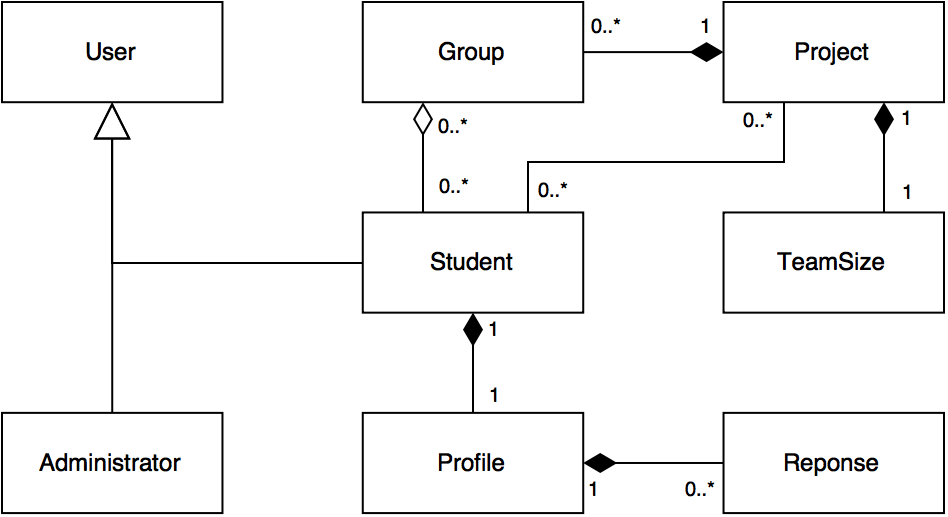
\includegraphics[scale=0.35]{imgs/entity-object-diagram.png}
	\caption{Entity Objects Diagram}
	\figurelabel{entity-obj}
\end{figure}

The following table, \tableref{entity-odd}, is the Data Dictionary for the Entity Objects. Here, we list out all the attributes and associations for each of the entity objects, as well as provide
a short but detailed definition of each.

\begin{table}[H]
	\caption{Entity Object Data Dictionary}\tablelabel{entity-odd}
	\begin{tabu} to \textwidth {l >{\bf}l X X[2.75]}
		\tableheader{}ID & Entity Object & Attributes/\newline Associations & Definition\\
		\cllabel{user}\clref{user} & User & 
		\begin{minipage}[t]{\linewidth}
			\begin{itemize}
				\item name
				\item id
			\end{itemize}
		\end{minipage} & 
		A \textbf{User} that has the ability to access the cuPID system.\\
		
		\cllabel{student}\clref{student} & Student & 
		\begin{minipage}[t]{\linewidth}
			\begin{itemize}
				\item studentNumber
				\item profile
			\end{itemize}
		\end{minipage} & 
		A \textbf{Student} is a specific type of User that can create/edit their Profiles and join/leave existing Projects.\\
		
		\cllabel{administrator}\clref{administrator} & Administrator & 
		&
		An \textbf{Administrator} is a specific type of user that can create/edit projects and run/view results of the PPID.\\

		\cllabel{group}\clref{group} & Group & 
		\begin{minipage}[t]{\linewidth}
			\begin{itemize}
				\item members
			\end{itemize}
		\end{minipage} & 
		A \textbf{Group} is a collection of Student Users that are participating in a specified Project. Every Project contains at least 1 Group, and the Students in a Group are decided when the Administrator runs the PPID algorithm.\\

		\cllabel{groupsize}\clref{groupsize} & GroupSize & 
		\begin{minipage}[t]{\linewidth}
			\begin{itemize}
				\item minSize
				\item maxSize
			\end{itemize}
		\end{minipage} & 
		The \textbf{GroupSize} contains the possible range of group sizes allowed such that the PPID algorithm will not make too big or too small groups.\\

		\cllabel{project}\clref{project} & Project & 
		\begin{minipage}[t]{\linewidth}
			\begin{itemize}
				\item name
				\item students
				\item groupSize
			\end{itemize}
		\end{minipage} & 
		A \textbf{Project} contains a collection of Students that will get sorted into Groups. These are made and edited by the \textbf{Administrator}.\\

		\cllabel{profile}\clref{profile} & Profile & 
		\begin{minipage}[t]{\linewidth}
			\begin{itemize}
				\item details
			\end{itemize}
		\end{minipage} & 
		A \textbf{Profile} is a set of responses maintained by each Student. These values are the necessary input for the PPID algorithm to run.\\
	\end{tabu}
\end{table}

\subsubsection*{Control and Boundary Objects}

Control objects are a special kind of object whose purpose is to fulfill use cases. In other words, the control objects are the objects that 
are doing all the tying together - they use function calls to access information from entity objects and create boundary objects to notify 
or interact with the actors (users). On the other hand, boundary objects are used to handle the interaction between actors and the system.
For example, if something erroneous has occurred, it is the boundary objects that notify the user.

\newpage{}

\subsubsection*{Control and boundary objects for ManageEnrollment (\ucref{manage-enrollment}):}

The following figure, \figureref{cbo-manage-enrollment}, handles the interactions between the control object, {\it ManageEnrollmentControl}, and the corresponding boundary objects, {\it ProjectListNotice, EnrollmentOption}, and {\it ProjectSelectionOption}. The control object here manages \ucref{manage-enrollment}, ManageEnrollment.

\vspace{1em}

\begin{figure}[H]
	\centering{}
	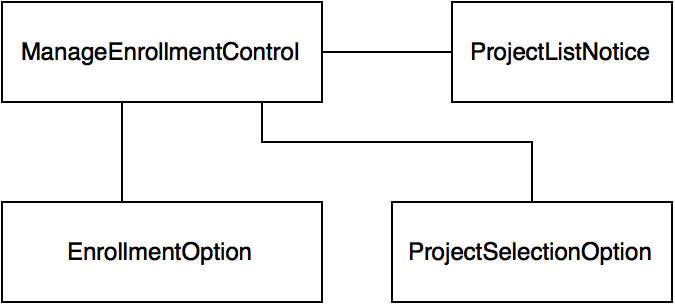
\includegraphics[scale=0.37]{imgs/cbod/manage-enrollment.png}
	\caption{Control/Boundary Objects for ManageEnrollment}
	\figurelabel{cbo-manage-enrollment}
\end{figure}

\subsubsection*{Control and boundary objects for EditProfile (\ucref{edit-profile}):}

The following figure, \figureref{cbo-edit-profile}, handles the interactions between the control object, {\it EditProfileControl}, and the corresponding
boundary object, {\it ProfileObject}. The control object here manages \ucref{edit-profile}, EditProfile.

\vspace{1em}

\begin{figure}[H]
	\centering{}
	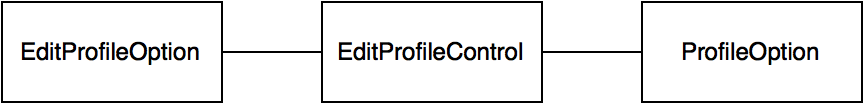
\includegraphics[scale=0.37]{imgs/cbod/edit-profile.png}
	\caption{Control/Boundary Objects for EditProfile}
	\figurelabel{cbo-edit-profile}
\end{figure}

\subsubsection*{Control and boundary objects for ManageProject (\ucref{manage-project}):}

The following figure, \figureref{cbo-edit-manage-project}, handles the interactions between the control object, {\it ManageProjectControl}, and the corresponding boundary objects, {\it ManageOption, ProjectListNotice,} and {\it ProjectSelectionOption}. The control object here manages \ucref{manage-project}, ManageProject.

\vspace{1em}

\begin{figure}[H]
	\centering{}
	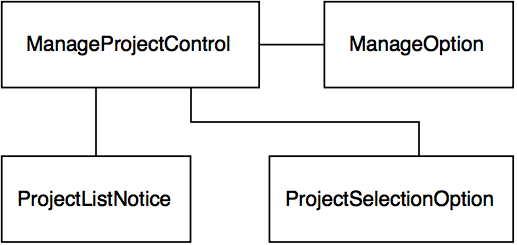
\includegraphics[scale=0.37]{imgs/cbod/manage-project.png}
	\caption{Control/Boundary Objects for ManageProject}
	\figurelabel{cbo-edit-manage-project}
\end{figure}

\newpage{}

\subsubsection*{Control and boundary objects for CreateNewProject (\ucref{create-new-project}):}

The following figure, \figureref{cbo-create-new-project}, handles the interactions between the control object, {\it CreateNewProjectControl}, and the corresponding boundary objects, {\it ProjectDetailsForm} and {\it ProjectCreateNotice}. The control object here manages \ucref{create-new-project}, CreateNewProject.

\begin{figure}[H]
	\centering{}
	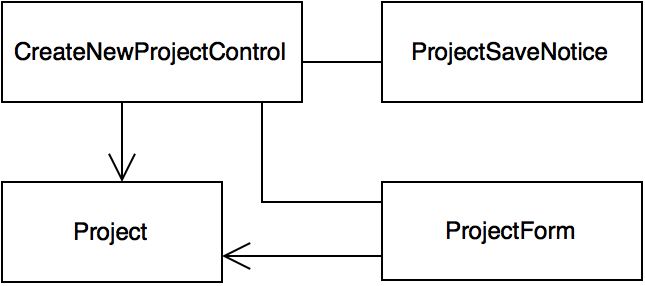
\includegraphics[scale=0.37]{imgs/cbod/create-new-project.png}
	\caption{Control/Boundary Objects for CreateNewProject}
	\figurelabel{cbo-create-new-project}
\end{figure}

\subsubsection*{Control and boundary objects for LaunchPPID (\ucref{launch-ppid}):}

The following figure, \figureref{cbo-launch-ppid}, handles the interactions between the control object, {\it LaunchPPIDControl}, the corresponding boundary object, {\it PPIDCompleteNotice}, and the entity object, {\it Project}. The control object here manages \ucref{launch-ppid}, LaunchPPID.

\begin{figure}[H]
	\centering{}
	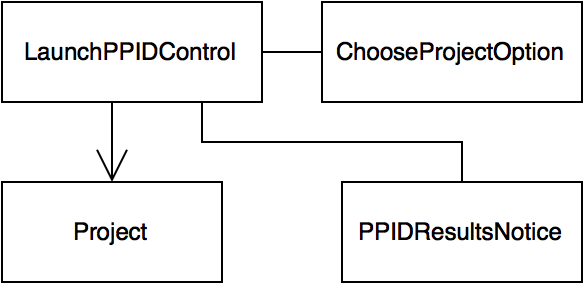
\includegraphics[scale=0.37]{imgs/cbod/launch-ppid.png}
	\caption{Control/Boundary Objects for LaunchPPID}
	\figurelabel{cbo-launch-ppid}
\end{figure}

\subsubsection*{Control and boundary objects for InsufficientStudentsError (\ucref{insufficient-students-error}):}

The following figure, \figureref{cbo-insufficient-students-error}, handles the interactions between the control objects, {\it LaunchPPIDControl} and {\it InsufficientStudentsErrorControl}, and the corresponding boundary object, {\it InsufficientStudentErrorNotice}. The control object here manages \ucref{insufficient-students-error}, InsufficientStudentsError.

\begin{figure}[H]
	\centering{}
	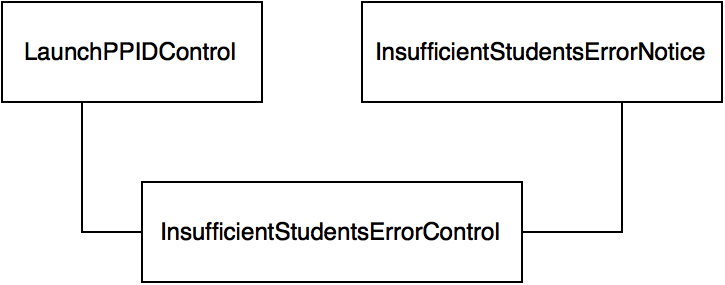
\includegraphics[scale=0.37]{imgs/cbod/insufficient-students-error.png}
	\caption{Control/Boundary Objects for InsufficientStudentsError}
	\figurelabel{cbo-insufficient-students-error}
\end{figure}

\newpage{}

\subsubsection*{Control and boundary objects for ViewPPIDResults (\ucref{view-ppid-results}):}

The following figure, \figureref{cbo-view-ppid-results}, handles the interactions between the control object, {\it ViewPPIDResultsControl} and the corresponding boundary object, {\it ResultsOption}. The control object here manages \ucref{view-ppid-results}, ViewPPIDResults.

\vspace{1em}

\begin{figure}[H]
	\centering{}
	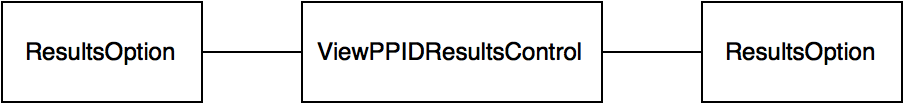
\includegraphics[scale=0.37]{imgs/cbod/view-ppid-results.png}
	\caption{Control/Boundary Objects for ViewPPIDResults}
	\figurelabel{cbo-view-ppid-results}
\end{figure}

\subsubsection*{Control and boundary objects for ViewPPIDSummary (\ucref{view-ppid-summary}):}

The following figure, \figureref{cbo-view-ppid-summary}, handles the interactions between the control object, {\it ViewPPIDSummaryControl}, the corresponding boundary object, 
{\it SummaryResultsNotice}, and the entity object, {\it Project}. The control object here manages \ucref{view-ppid-summary}, ViewPPIDSummary.

\vspace{1em}

\begin{figure}[H]
	\centering{}
	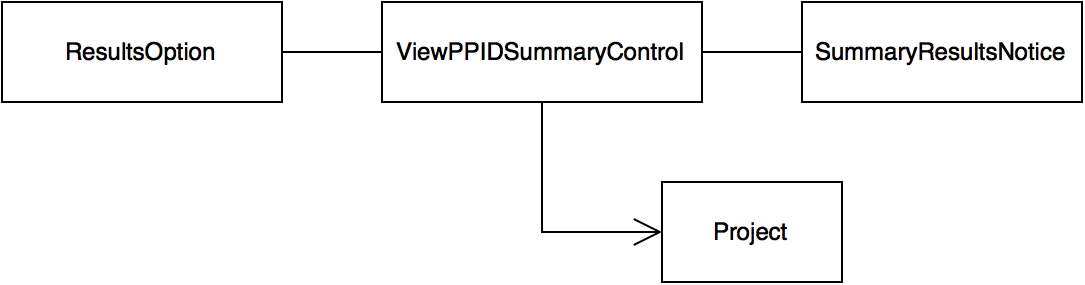
\includegraphics[scale=0.37]{imgs/cbod/view-ppid-summary.png}
	\caption{Control/Boundary Objects for ViewPPIDSummary}
	\figurelabel{cbo-view-ppid-summary}
\end{figure}

\subsubsection*{Control and boundary objects for ViewPPIDDetails (\ucref{view-ppid-details}):}

The following figure, \figureref{cbo-view-ppid-details}, handles the interactions between the control object, {\it ViewPPIDDetailsControl}, the corresponding boundary object, 
{\it DetailsResultsNotice}, and the entity object, {\it Project}. The control object here manages \ucref{view-ppid-details}, ViewPPIDDetails.

\vspace{1em}

\begin{figure}[H]
	\centering{}
	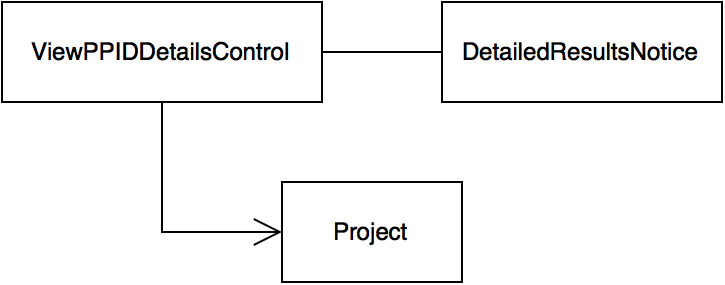
\includegraphics[scale=0.37]{imgs/cbod/view-ppid-details.png}
	\caption{Control/Boundary Objects for ViewPPIDDetails}
	\figurelabel{cbo-view-ppid-details}
\end{figure}

\newpage{}

\subsubsection*{Control and boundary objects for EditProjectDetails (\ucref{edit-project-details}):}

The following figure, \figureref{cbo-edit-project-details}, handles the interactions between the control object, {\it EditProjectDetailsControl}, the corresponding boundary objects, {\it ProjectDetailsForm} and {\it DetailsUpdateNotice}, and the entity object, {\it Project}. The control object here manages \ucref{edit-project-details}, EditProjectDetails.

\begin{figure}[H]
	\centering{}
	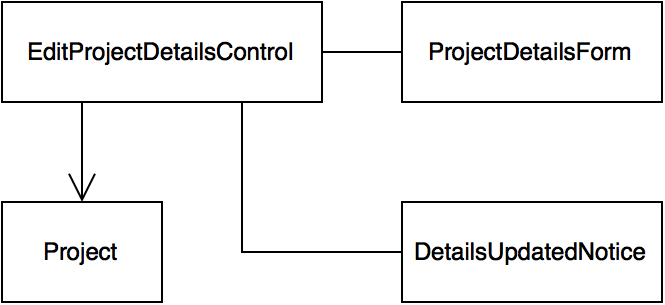
\includegraphics[scale=0.37]{imgs/cbod/edit-project-details.png}
	\caption{Control/Boundary Objects for EditProjectDetails}
	\figurelabel{cbo-edit-project-details}  
\end{figure}

\subsubsection*{Control and boundary objects for EditProject (\ucref{edit-project}):}

The following figure, \figureref{cbo-edit-project}, handles the interactions between the control object, {\it EditProjectControl} and the corresponding boundary objects, 
{\it ProjectDetailsForm} and {\it DetailsUpdateNotice}. The control object here manages \ucref{edit-project}, EditProject.

\begin{figure}[H]
	\centering{}
	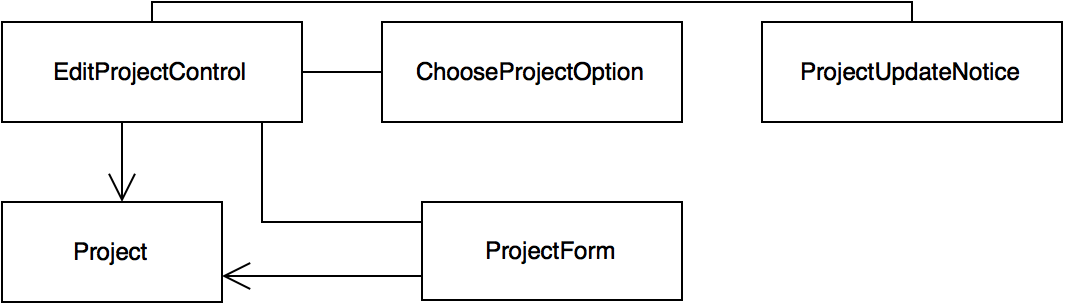
\includegraphics[scale=0.37]{imgs/cbod/edit-project.png}
	\caption{Control/Boundary Objects for EditProject}
	\figurelabel{cbo-edit-project}
\end{figure}

\subsubsection*{Control and boundary objects for JoinProject (\ucref{join-project}):}

The following figure, \figureref{cbo-join-project}, handles the interactions between the control object, {\it JoinProjectControl}, the corresponding boundary objects, 
{\it EnrollmentOption} and {\it JoinCompleteNotice}, and the entity object, {\it Project}. The control object here manages \ucref{join-project}, JoinProject.

\begin{figure}[H]
	\centering{}
	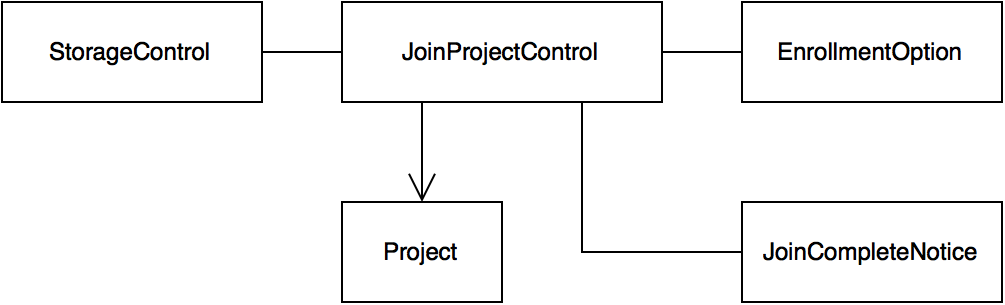
\includegraphics[scale=0.37]{imgs/cbod/join-project.png}
	\caption{Control/Boundary Objects for JoinProject}
	\figurelabel{cbo-join-project}    
\end{figure}

\newpage{}

\subsubsection*{Control and boundary objects for LeaveProject (\ucref{leave-project}):}

The following figure, \figureref{cbo-leave-project}, handles the interactions between the control object, {\it LeaveProjectControl}, the corresponding boundary objects, 
{\it ProjectDetailsForm} and {\it LeaveCompleteNotice}, and the entity object, {\it Project}. The control object here manages \ucref{leave-project}, LeaveProject.

\begin{figure}[H]
	\centering{}
	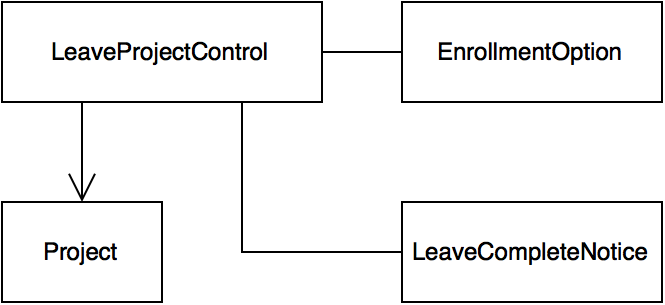
\includegraphics[scale=0.37]{imgs/cbod/leave-project.png}
	\caption{Control/Boundary Objects for LeaveProject}
	\figurelabel{cbo-leave-project}
\end{figure}

\subsubsection*{Control and boundary objects for EditPersonalValues (\ucref{edit-personal-values}):}

The following figure, \figureref{cbo-edit-personal-values}, handles the interactions between the control object, {\it EditPersonalValues}, the corresponding boundary objects, {\it ProfileOption} and {\it UpdateCompleteNotice}, and the entity object, {\it Student}. The control object here manages \ucref{edit-personal-values}, EditPersonalValues.

\begin{figure}[H]
	\centering{}
	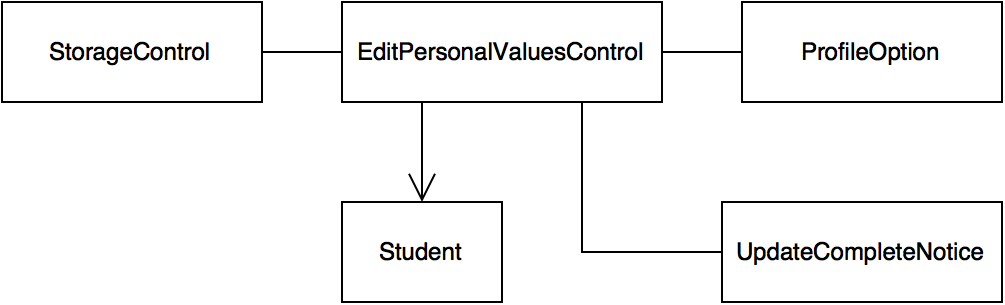
\includegraphics[scale=0.37]{imgs/cbod/edit-personal-values.png}
	\caption{Control/Boundary Objects for EditPersonalValues}
	\figurelabel{cbo-edit-personal-values}
\end{figure}

\subsubsection*{Control and boundary objects for EditDesiredValues (\ucref{edit-desired-values}):}

The following figure, \figureref{cbo-edit-desired-values}, handles the interactions between the control object, {\it EditDesiredValues}, the corresponding boundary objects, {\it ProfileOption} and {\it UpdateCompleteNotice}, and the entity object, {\it Student}. The control object here manages \ucref{edit-desired-values}, EditDesiredValues.

\begin{figure}[H]
	\centering{}
	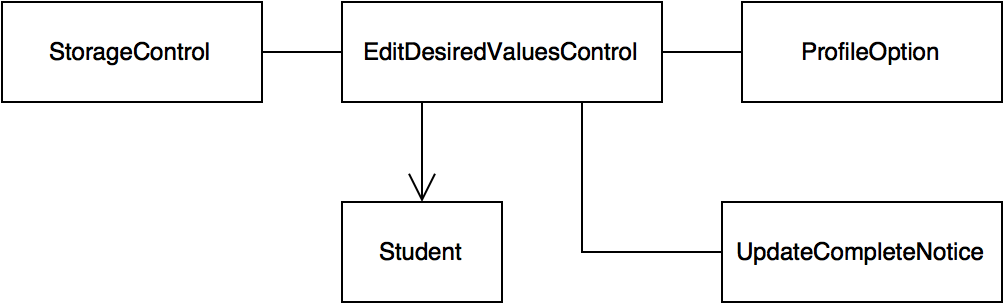
\includegraphics[scale=0.37]{imgs/cbod/edit-desired-values.png}
	\caption{Control/Boundary Objects for EditDesiredValues}
	\figurelabel{cbo-edit-desired-values}
\end{figure}

\newpage{}

\subsubsection*{Control and boundary objects for InvalidInputError (\ucref{invalid-input-error}):}

The following figure, \figureref{cbo-invalid-input-error}, handles the interactions between the control object, {\it InvalidInputErrorControl} and the corresponding boundary objects, {\it InputOption} and {\it InvalidInputErrorNotice}. The control object here manages \ucref{invalid-input-error}, InvalidInputError.

\begin{figure}[H]
	\centering{}
	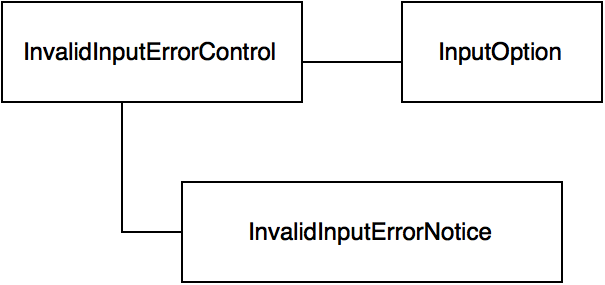
\includegraphics[scale=0.37]{imgs/cbod/invalid-input-error.png}
	\caption{Control/Boundary Objects for InvalidInputError}
	\figurelabel{cbo-invalid-input-error}
\end{figure}

\subsubsection*{Control and boundary objects for EditProjectName (\ucref{edit-project-name}):}

The following figure, \figureref{cbo-edit-project-name}, handles the interactions between the control object, {\it EditProjectNameControl}, the corresponding boundary objects, {\it EditProjectNameOption} and {\it ProjectNameUpdateNotice}, and the entity object, {\it Project}. The control object here manages \ucref{edit-project-name}, EditProjectName.

\begin{figure}[H]
	\centering{}
	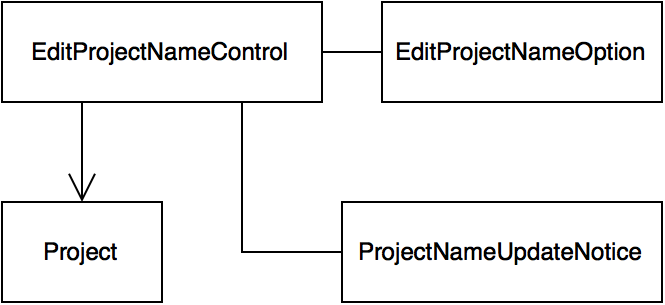
\includegraphics[scale=0.37]{imgs/cbod/edit-project-name.png}
	\caption{Control/Boundary Objects for EditProjectName}
	\figurelabel{cbo-edit-project-name}
\end{figure}

\subsubsection*{Control and boundary objects for ProjectExistsError (\ucref{project-exists-error}):}

The following figure, \figureref{cbo-project-exists-error}, handles the interactions between the control objects, {\it EditProjectDetailsControl} and {\it ProjectExistsErrorControl}, and the corresponding boundary object, {\it ProjectExistsErrorNotice}. The control object here manages \ucref{project-exists-error}, ProjectExistsError.

\begin{figure}[H]
	\centering{}
	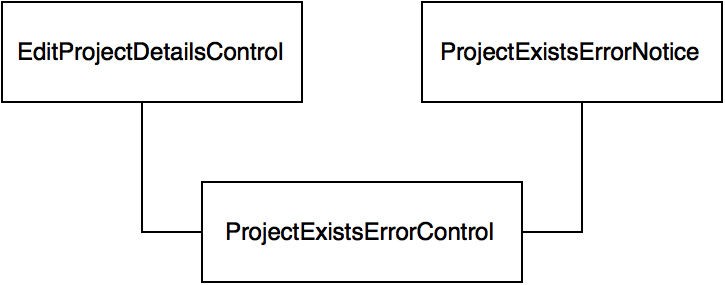
\includegraphics[scale=0.37]{imgs/cbod/project-exists-error.png}
	\caption{Control/Boundary Objects for ProjectExistsError}
	\figurelabel{cbo-project-exists-error}
\end{figure}

\newpage{}

\subsubsection*{Control and boundary objects for EditGroupSize (\ucref{edit-group-size}):}

The following figure, \figureref{cbo-edit-group-size}, handles the interactions between the control object, {\it EditGroupSizeControl}, the corresponding boundary objects, 
{\it EditGroupSizeOption} and {\it GroupSizeUpdateNotice}, and the entity object, {\it Project}. The control object here manages \ucref{edit-group-size}, EditGroupSize.

\begin{figure}[H]
	\centering{}
	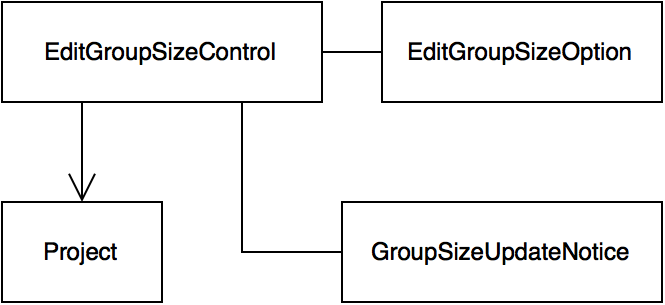
\includegraphics[scale=0.37]{imgs/cbod/edit-group-size.png}
	\caption{Control/Boundary Objects for EditGroupSize}
	\figurelabel{cbo-edit-group-size}
\end{figure}

\subsubsection*{Control and boundary objects for InvalidGroupSizeError (\ucref{invalid-group-size-error}):}

The following figure, \figureref{cbo-invalid-group-size}, handles the interactions between the control objects, {\it EditGroupSizeControl} and {\it InvalidGroupSizeErrorControl}, and the corresponding boundary object, {\it InvalidGroupSizeErrorNotice}. The control object here manages \ucref{invalid-group-size-error}, InvalidGroupSizeError.

\begin{figure}[H]
	\centering{}
	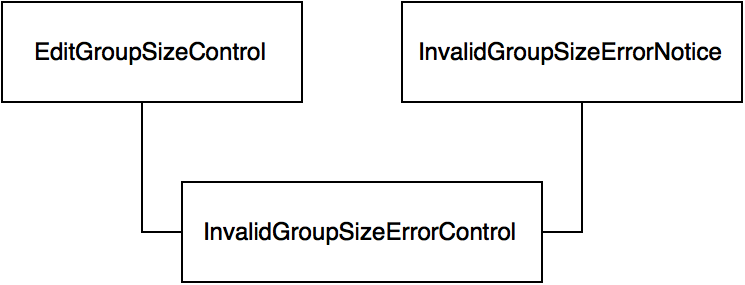
\includegraphics[scale=0.37]{imgs/cbod/invalid-group-size-error.png}
	\caption{Control/Boundary Objects for InvalidGroupSizeError}
    \figurelabel{cbo-invalid-group-size}
\end{figure}

\subsubsection*{Control and boundary objects for StorageError (\ucref{storage-error}):}

The following figure, \figureref{cbo-storage-error}, handles the interactions between the control objects, {\it StorageControl} and {\it StorageErrorControl}, and the corresponding boundary object, 
{\it StorageErrorNotice}. The control object here manages \ucref{storage-error}, StorageError.

\begin{figure}[H]
	\centering{}
	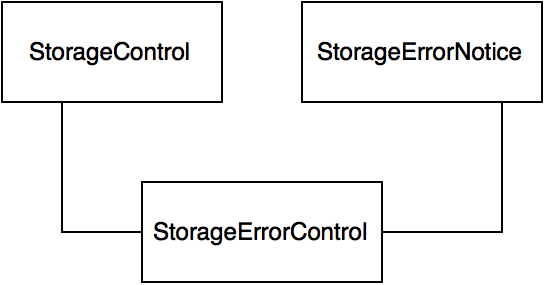
\includegraphics[scale=0.37]{imgs/cbod/storage-error.png}
	\caption{Control/Boundary Objects for StorageError}
	\figurelabel{cbo-storage-error}
\end{figure}

\newpage{}

\subsubsection*{Control and boundary objects for StorageReadError (\ucref{storage-read-error}):}

The following figure, \figureref{cbo-storage-read-error}, handles the interactions between the control objects, {\it StorageControl} and {\it StorageReadErrorControl}, and the corresponding boundary object, 
{\it StorageReadErrorNotice}. The control object here manages \ucref{storage-read-error}, StorageReadError.

\begin{figure}[H]
	\centering{}
	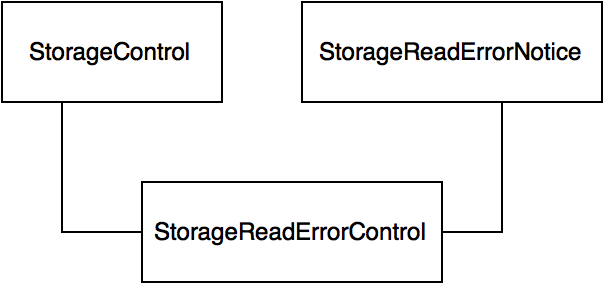
\includegraphics[scale=0.37]{imgs/cbod/storage-read-error.png}
	\caption{Control/Boundary Objects for StorageReadError}
	\figurelabel{cbo-storage-read-error}
\end{figure}

\subsubsection*{Control and boundary objects for StorageOpenError (\ucref{storage-open-error}):}

The following figure, \figureref{cbo-storage-open-error}, handles the interactions between the control objects, {\it StorageControl} and {\it StorageOpenErrorControl}, and the corresponding boundary object, 
{\it StorageOpenErrorNotice}. The control object here manages \ucref{storage-open-error}, StorageOpenError.

\begin{figure}[H]
	\centering{}
	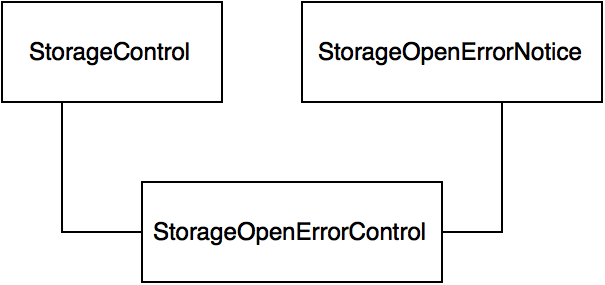
\includegraphics[scale=0.37]{imgs/cbod/storage-open-error.png}
	\caption{Control/Boundary Objects for StorageOpenError}
	\figurelabel{cbo-storage-open-error}
\end{figure}

\subsubsection*{Control and boundary objects for StorageWriteError (\ucref{storage-write-error}):}

The following figure, \figureref{cbo-storage-write-error}, handles the interactions between the control objects, {\it StorageControl} and {\it StorageWriteErrorControl}, and the corresponding boundary object, {\it StorageWriteErrorNotice}. The control object here manages \ucref{storage-write-error}, StorageWriteError.

\begin{figure}[H]
	\centering{}
	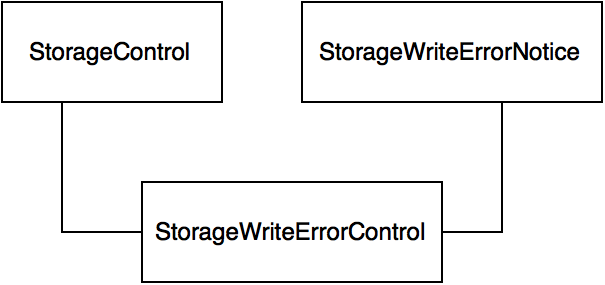
\includegraphics[scale=0.37]{imgs/cbod/storage-write-error.png}
	\caption{Control/Boundary Objects for StorageWriteError}
	\figurelabel{cbo-storage-write-error}
\end{figure}

The following table, \tableref{control-odd}, is the Data Dictionary for the control objects. It contains all the control objects shown in the above diagrams, each coupled with a very detailed definition. 
This definition includes details such as what use case each control object manages and when/how each control objects are created.

\begin{table}[H]
\caption{Control Object Data Dictionary}\tablelabel{control-odd}
	\begin{tabu} to \textwidth {l >{\bf}X X[3]}
		\tableheader{}ID & Control Object & Definition\\
		\cllabel{manage-enrollment-ctrl}\clref{manage-enrollment-ctrl} & Manage\-Enrollment\-Control & 
			The {\bf ManageEnrollmentControl} object manages the ManageEnrollment use case. This object is created when the Student user
			selects the ManageEnrollmentOption.  It displays a list of all the available Projects for the Student to choose from. Upon choosing, the
			Student will then be given the options of either joining or leaving a project. \\
		
		\cllabel{edit-profile-ctrl}\clref{edit-profile-ctrl} & Edit\-Profile\-Control & 
			The {\bf EditProfileControl} object manages the EditProfile use case. This object is created when the Student user selects the EditProfileOption.
			It provides the Student the option to edit/modify either their personal values or their desired values for their Profile. Depending on the response, control is then
			handed over to either the EditPersonalValuesControl or the EditDesiredValuesControl objects. \\
		
		\cllabel{manage-project-ctrl}\clref{manage-project-ctrl} & Manage\-Project\-Control & 
			The {\bf ManageProjectControl} object manages the ManageProject use case. This object is created after the Administrator user selects the
			ManageProjectOption. It provides the Administrator the option to select a Project and modify details for that Project. Depending on which detail
			is selected, control is then handed over to either the LaunchPPIDControl, the ViewPPIDResultsControl, or the EditProjectControl objects.\\
		
		\cllabel{create-new-project-ctrl}\clref{create-new-project-ctrl} & Create\-New\-Project\-Control & 
			The {\bf CreateNewProjectControl} object manages the CreateNewProject use case. This object is created after the Administrator user selects the
			CreateNewProjectOption. It provides the Administrator with the ability to create new Projects, including the filling in of the details for this new project,
			which is managed by the EditProjectControl object. The notice, ProjectCreateNotice, is then displayed.\\
		
		\cllabel{launch-ppid-ctrl}\clref{launch-ppid-ctrl} & Launch\-PPID\-Control & 
			The {\bf LaunchPPIDControl} object manages the LaunchPPID use case. This object is created after the Administrator launches the PPID from
			the ManageProjectOption. It cycles through the list of currently enrolled students in the Project and sorts them into teams. The result is then saved
			to the Storage and a notice, PPIDCompleteNotice, is displayed.\\
	\end{tabu}
\end{table}

\begin{center}
\begin{tabu} to \textwidth {l >{\bf}X X[3]}
		\tableheader{}ID & Control Object & Definition\\
		\cllabel{insufficient-students-error-ctrl}\clref{insufficient-students-error-ctrl} & Insufficient\-StudentsError\-Control & 
			The {\bf InsufficientStudentsErrorControl} object manages the InsufficientStudentsError use case. The object is created when the Administrator user
			tries to run the PPID when the amount of Students enrolled is less than the minimum team size specified for the Project. A notice, InsufficientStudentsErrorNotice,
			is displayed and the operation is cancelled.\\
		
		\cllabel{view-ppid-results-ctrl}\clref{view-ppid-results-ctrl} & View\-PPID\-Results\-Control & 
			The {\bf ViewPPIDResultsControl} object manages the ViewPPIDResults use case. The object is created when the Administrator user selects the
			ViewPPIDResultsOption. It provides the Administrator with two options for displaying the results of the last run PPID - either in simple form, where the
			groups are simply printed out, or in detailed form, where the reasoning for the groups is also printed out. Depending on which gets selected, control is then
			handed off to either the ViewPPIDSummaryControl or the ViewPPIDDetailsControl objects.\\
		
		\cllabel{view-ppid-summary-ctrl}\clref{view-ppid-summary-ctrl} & View\-PPID\-Summary\-Control & 
			The {\bf ViewPPIDSummaryControl} object manages the ViewPPIDSummary use case. The object is created when the Administrator user selects Summary from the
			two options provided in the ResultsOption object. It displays to the Administrator a print out of all the groups that the last run PPID created in a simple, easy to
			read manner.\\
		
		\cllabel{view-ppid-details-ctrl}\clref{view-ppid-details-ctrl} & View\-PPID\-Details\-Control & 
			The {\bf ViewPPIDDetailsControl} object manages the ViewPPIDDetails use case. The object is created when the Administrator user selects Detailed from the two 
			options provided in the ResultsOption object. It displays to the Administrator a detailed print out of the reasoning and steps with regards to the last PPID run.\\
		
		\cllabel{edit-project-details-ctrl}\clref{edit-project-details-ctrl} & Edit\-Project\-Details\-Control & 
			The {\bf EditProjectDetailsControl} object manages the EditProjectDetails use case. The object is created after the Administrator user inputs the new details into
			the ProjectDetailsForm and submits it. It then updates the values in the Project object and saves the updated Project to the Storage. A notice, DetailsUpdatedNotice,
			is then displayed to the Administrator.\\
		
		\cllabel{edit-project-ctrl}\clref{edit-project-ctrl} & Edit\-Project\-Control & 
			The {\bf EditProjectControl} object manages the EditProject use case. The object is created after the Administrator user selects the EditProjectOption. It then
			creates a ProjectDetailsForm for the user to fill in. Control is then passed over to the EditProjectDetailsControl object.\\
\end{tabu}
\end{center}

\begin{center}
\begin{tabu} to \textwidth {l >{\bf}X X[3]}
		\tableheader{}ID & Control Object & Definition\\
		\cllabel{join-project-ctrl}\clref{join-project-ctrl} & Join\-Project\-Control & 
			The {\bf JoinProjectControl} object manages the JoinProject use case. The object is created when the Student user selects Join from the two options provided
			in the EnrollmentOption object. It allows the Student to join an existing Project, then updates that Project and saves the updated Project to the Storage. Finally, 
			a notice, JoinCompleteNotice, is displayed to the Student.\\
		
		\cllabel{leave-project-ctrl}\clref{leave-project-ctrl} & Leave\-Project\-Control & 
			The {\bf LeaveProjectControl} object manages the LeaveProject use case. The object is created when the Student user selects Leave from the two options provided
			in the EnrollmentOption object. It allows the Student to leave a Project that they are already a part of, then updates that Project and saves the updated Project to
			the Storage. Finally, a notice, LeaveCompleteNotice, is displayed to the Student.\\
		
		\cllabel{edit-personal-values-ctrl}\clref{edit-personal-values-ctrl} & Edit\-Personal\-Values\-Control & 
			The {\bf EditPersonalValuesControl} object manages the EditPersonalValues use case. The object is created when the Student selects PersonalValues from the two
			options provided by the ProfileOption object. It allows the Student to input new responses for the Personal Values section of their Profile, then updates the Student
			object and saves the updated Student object to the Storage. Finally, a notice, UpdateCompleteNotice, is displayed to the Student.\\
		
		\cllabel{edit-desired-values-ctrl}\clref{edit-desired-values-ctrl} & Edit\-Desired\-Values\-Control & 
			The {\bf EditDesiredValuesControl} object manages the EditDesiredValues use case. The object is created when the Student selects DesiredValues from the two
			options provided by the ProfileOption object. It allows the Student to input new response for the Desired Values section of their Profile, then updates the Student
			object and saves the updated Student object to the Storage. Finally, a notice, UpdateCompleteNotice, is displayed to the Student. \\
		
		\cllabel{invalid-input-error-ctrl}\clref{invalid-input-error-ctrl} & Invalid\-Input\-Error\-Control & 
			The {\bf InvalidInputErrorControl} object manages the InvalidInputError use case. The object is created when the Administrator inputs invalid data. It creates a notice, 
			InvalidInputErrorNotice, and displays it to the Administrator. The input operation is then cancelled.\\

		\cllabel{edit-project-name-ctrl}\clref{edit-project-name-ctrl} & Edit\-Project\-Name\-Control & 
			The {\bf EditProjectNameControl} object manages the EditProjectName use case. The object is created when the Administrator selects the EditProjectNameOption.
			It then updates the Project object and saves the updated Project object to the Storage. Finally, a notice, ProjectNameUpdateNotice, is displayed to the Administrator.\\
\end{tabu}
\end{center}

\begin{center}
\begin{tabu} to \textwidth {l >{\bf}X X[3]}
		\tableheader{}ID & Control Object & Definition\\
		\cllabel{project-exists-error-ctrl}\clref{project-exists-error-ctrl} & Project\-Exists\-Error\-Control &
			The {\bf ProjectExistsErrorControl} object manages the ProjectExistsError use case. The object is created when Administrator users attempt to set 
			the Project name to a name that alread exists. A notice, ProjectExistsErrorNotice, is displayed to the Administrator, and the EditProjectName operation is cancelled.\\
		
		\cllabel{edit-group-size-ctrl}\clref{edit-group-size-ctrl} & Edit\-Group\-Size\-Control & 
			The {\bf EditGroupSizeControl} object manages the EditGroupSize use case. The object is created when the Administrator user selects the EditGroupSizeOption. It allows the 
			Administrator to input a new Maximum and Minimum group size value and updates the Project object. Finally, a notice, GroupSizeUpdateNotice, is displayed to the Administrator.\\
		
		\cllabel{invalid-group-size-error-ctrl}\clref{invalid-group-size-error-ctrl} & Invalid\-Group\-Size\-Error\-Control & 
			The {\bf InvalidGroupSizeErrorControl} object manages the InvalidGroupSizeError use case. The object is created when the Administrator attempts to input an invalid size for the Maximum
			and Minimum group size variables. A notice, InvalidGroupSizeErrorNotice, is displayed to the Administrator, and the EditGroupSize operation is cancelled. \\
		
		\cllabel{storage-ctrl}\clref{storage-ctrl} & Storage\-Control & 
			The {\bf StorageControl} object manages...\\
		
		\cllabel{storage-error-ctrl}\clref{storage-error-ctrl} & Storage\-Error\-Control & 
			The {\bf StorageErrorControl} object manages the StorageError use case. The object is created when any user makes a request to the Storage and the request cannot be met.
			It then displays a notice, StorageErrorNotice, to the user.\\
\end{tabu}
\end{center}

\begin{center}
\begin{tabu} to \textwidth {l >{\bf}X X[3]}
		\tableheader{}ID & Control Object & Definition\\
		\cllabel{storage-read-error-ctrl}\clref{storage-read-error-ctrl} & Storage\-Read\-Error\-Control & The {\bf StorageReadErrorControl} object manages the StorageReadError use case. The object is created when any user makes a request to read a file from the Storage and the read operation fails. It then displays a notice, StorageReadErrorNotice, to the user.\\

		\cllabel{storage-open-error-ctrl}\clref{storage-open-error-ctrl} & Storage\-Open\-Error\-Control & The {\bf StorageOpenErrorControl} object manages the StorageOpenError use case. The object is created when any user makes a request to open the Storage and the operation fails. It then displays a notice, StorageOpenErrorNotice, to the user.\\

		\cllabel{storage-write-error-ctrl}\clref{storage-write-error-ctrl} & Storage\-Write\-Error\-Control & object manage the StorageWriteError use case. The object is created when any user makes a write to the Storage request and the operation fails. It then displays a notice, StorageWriteErrorNotice, to the user.\\
\end{tabu}
\end{center}

\newpage{}

The following table, \tableref{boundary-odd}, is the Data Dictionary for the boundary objects. It contains all the boundary objects shown in the above diagrams, each coupled with a detailed definition.
In essence, the definition explains what each object does.

\begin{table}[H]
    \caption{Boundary Object Data Dictionary}\tablelabel{boundary-odd}
	\begin{tabu} to \textwidth {l >{\bf}X X[3]}
		\tableheader{}ID & Boundary Object & Definition\\
		\cllabel{project-list-notice}\clref{project-list-notice} & Project\-List\-Notice & 
			This object is responsible for the visual output of the list of Projects to the User. It gets the required information from the Project objects and displays it.\\
		
		\cllabel{enrollment-option}\clref{enrollment-option} & Enrollment\-Option & 
			This object allows the Student to view and choose between the two enrollment options: Join or Leave.\\
		
		\cllabel{project-selection-option}\clref{project-selection-option} & Project\-Selection\-Option & 
			This object reads the selected Project from the Administrator.\\
		
		\cllabel{profile-option}\clref{profile-option} & Profile\-Option & 
			This object allows the Student to view and choose between the two profile options: edit Personal Details or edit Desired Details.\\
		
		\cllabel{manage-option}\clref{manage-option} & Manage\-Option & 
			This object allows the Administrator to view and choose between three managing options: view the results of the last PPID, edit a project, or delete a project.\\
		
		\cllabel{project-create-notice}\clref{project-create-notice} & Project\-Create\-Notice & 
			This object displays a notice to the Administrator stating that the Project has been successfully created.\\
		
		\cllabel{project-details-form}\clref{project-details-form} & Project\-Details\-Form & 
			This object is a form that reads the inputted values from the Administrator for the Project details.\\
		
		\cllabel{ppid-complete-notice}\clref{ppid-complete-notice} & PPID\-Complete\-Notice & 
			This object displays a notice to the Administrator stating that the PPID has run successfully.\\
		
		\cllabel{insufficient-student-error-notice}\clref{insufficient-student-error-notice} & Insufficient\-Student\-Error\-Notice & 
			This object displays a notice to the Administrator stating that the PPID has failed due to an insufficient amount of students enrolled in the Project.\\
		
		\cllabel{results-option}\clref{results-option} & Results\-Option & 
			This object allows the Administrator to view and choose between the two result options: Summary or Detailed.\\
		
		\cllabel{summary-results-notice}\clref{summary-results-notice} & Summary\-Results\-Notice & 
			This object displays a notice to the Administrator that shows the simple summary print out of the Groups.\\
		
		\cllabel{detailed-results-notice}\clref{detailed-results-notice} & Detailed\-Results\-Notice & 
			This object displays a notice to the Administrator that shows the detailed print out of the Groups and the reasoning that the algorithm had when making the decisions.\\
		
		\cllabel{details-update-notice}\clref{details-update-notice} & Details\-Updated\-Notice & 
			This object displays a notice to the Administrator stating that the saving of the new Project details to Storage was successful.\\
	\end{tabu}
\end{table}

\begin{center}
\begin{tabu} to \textwidth {l >{\bf}X X[3]}
		\tableheader{}ID & Boundary Object & Definition\\
		\cllabel{project-update-notice}\clref{project-update-notice} & Project\-Update\-Notice & 
			This object displays a notice to the Administrator stating that the editing of the Project has been completed successfully\\
		
		\cllabel{join-complete-notice}\clref{join-complete-notice} & Join\-Complete\-Notice & 
			This object displays a notice to the Student stating that the joining of a Project was successful.\\
		
		\cllabel{leave-complete-notice}\clref{leave-complete-notice} & Leave\-Complete\-Notice & 
			This object displays a notice to the Student stating that the leaving of a Project was successful.\\
		
		\cllabel{update-complete-notice}\clref{update-complete-notice} & Update\-Complete\-Notice & 
			This object displays a notice to the Student stating that the saving of the new Profile details (either Personal values or Desired values) to the Storage was successful.\\
		
		\cllabel{input-option}\clref{input-option} & Input\-Option & 
			This object reads the input from the Administrator.\\ %double check this one!
		
		\cllabel{invalid-input-error-notice}\clref{invalid-input-error-notice} & Invalid\-Input\-Error\-Notice & 
			This object displays a notice to the Administrator stating that the input given was invalid.\\
		
		\cllabel{edit-project-name-option}\clref{edit-project-name-option} & Edit\-Project\-Name\-Option & 
			This object reads the input from the Administrator for the new Project Name field.\\
		
		\cllabel{project-name-update-notice}\clref{project-name-update-notice} & Project\-Name\-Update\-Notice & 
			This object displays a notice to the Administrator stating that the updating/setting of the Project name has been successful.\\
		
		\cllabel{project-exists-error-notice}\clref{project-exists-error-notice} & Project\-Exists\-Error\-Notice & 
			This object displays a notice to teh Administrator stating that the desired Project name has already been taken.\\
		
		\cllabel{edit-group-size-option}\clref{edit-group-size-option} & Edit\-Group\-Size\-Option & 
			This object reads the input from the Administrator for the Maximum and Minimum group size fields.\\
		
		\cllabel{group-size-update-notice}\clref{group-size-update-notice} & Group\-Size\-Update\-Notice & 
			This object displays a notice to the Administrator stating that the group size has been successfully updated.\\
		
		\cllabel{invalid-group-size-error-notice}\clref{invalid-group-size-error-notice} & Invalid\-Group\-Size\-Error\-Notice & 
			This object displays a notice to the Administrator stating that the given value for the group size is invalid.\\
		
		\cllabel{storage-error-notice}\clref{storage-error-notice} & Storage\-Error\-Notice & 
			This object displays a notice to the User stating that there was an error with the request to the Storage.\\
		
		\cllabel{storage-read-error-notice}\clref{storage-read-error-notice} & Storage\-Read\-Error\-Notice & 
			This object displays a notice to the User stating that there was an error with regards to reading a file from Storage.\\
		
		\cllabel{storage-open-error-notice}\clref{storage-open-error-notice} & Storage\-Open\-Error\-Notice & 
			This object displays a notice to the User stating that there was an error with regards to opening the Storage.\\
		
		\cllabel{storage-write-error-notice}\clref{storage-write-error-notice} & Storage\-Write\-Error\-Notice & 
			This object displays a notice to the User stating that there was an error with regards to writing to the Storage.\\
\end{tabu}
\end{center}

\newpage{}

\subsubsection{Dynamic Model}

Dynamic models serve to represent how a system works or behaves from an outside point-of-view. There will be two different types of dynamic
models in this section: state machines and sequence diagrams. State machines are very particular in the sense that they will only represent the 
behavior of a single object. For this project, only the entity state machines are shown. Sequence diagrams are different in the sense that they
provide a visual representation of the interactions between multiple objects for the fulfillment of a single use case.

\subsubsection*{State Machines}

State machines are a special kind of dynamic model that shows all the possible states of a single object. Also shown in here is the interaction between these 
different states - that is, how it goes from one state to the other. The starting and ending points, or beginning and exit points, are also shown. Specifically, these state
machines only concern entity objects for this particular project.

\subsubsection*{State Machines for User/Student/Administrator:}

The following diagram, \figureref{sm-user-log-in}, represents a state machine for any type of User object. Shown here is the different states involved in logging in/logging out.

\begin{figure}[H]
    \smlabel{user-log-in}
	\centering{}
	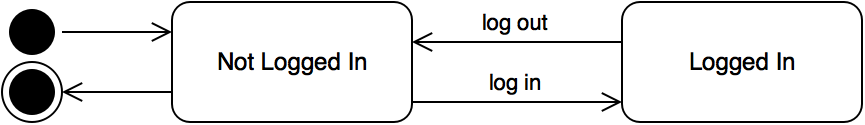
\includegraphics[scale=0.3]{imgs/state/user-log-in.png}
	\caption[\smref{user-log-in} - State Machine for User/Student/Administrator Login]{State Machine for User/Student/Administrator Login (\smref{user-log-in})}
	\figurelabel{sm-user-log-in}
\end{figure}

\subsubsection*{State Machines for Student:}

The following diagram, \figureref{sm-student-join-project}, represents a state machine for the Student object. Shown here is the different states involved in the joining of Projects.

\begin{figure}[H]
    \smlabel{student-join-project}
	\centering{}
	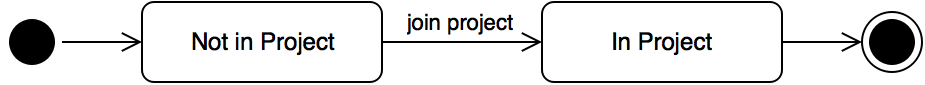
\includegraphics[scale=0.3]{imgs/state/student-join-project.png}
	\caption[\smref{student-join-project} - State Machine for Student Join Project]{State Machine for Student Join Project (\smref{student-join-project})}
	\figurelabel{sm-student-join-project}
\end{figure}

\noindent The following diagram, \figureref{sm-student-leave-project}, represents a state machine for the Student object. Shown here is the different states involved in the leaving of Projects.

\begin{figure}[H]
    \smlabel{student-leave-project}
	\centering{}
	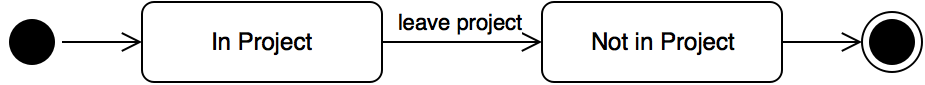
\includegraphics[scale=0.3]{imgs/state/student-leave-project.png}
	\caption[\smref{student-leave-project} - State Machine for Student Leave Project]{State Machine for Student Leave Project (\smref{student-leave-project})}
	\figurelabel{sm-student-leave-project}
\end{figure}

\newpage{}

\subsubsection*{State Machines for Profile:}

The following diagram, \figureref{sm-profile-details}, represents a state machine for the Profile object. Shown here is the different states involved in managing profile details.

\begin{figure}[H]
    \smlabel{profile-details}
	\centering{}
	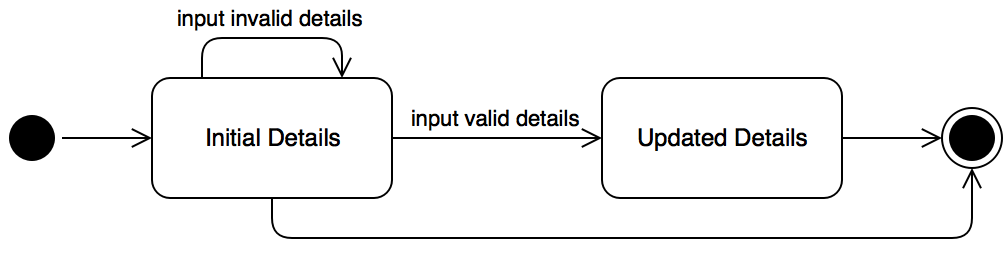
\includegraphics[scale=0.3]{imgs/state/profile-details.png}
	\caption[\smref{profile-details} - State Machine for Profile Details]{State Machine for Profile Details (\smref{profile-details})}
	\figurelabel{sm-profile-details}
\end{figure}

\subsubsection*{State Machines for Project:}

The following diagram, \figureref{sm-project-student-enrollment}, represents a state machine for the Project object. Shown here is the different states involved in the adding and removing Students.

\begin{figure}[H]
    \smlabel{project-student-enrollment}
	\centering{}
	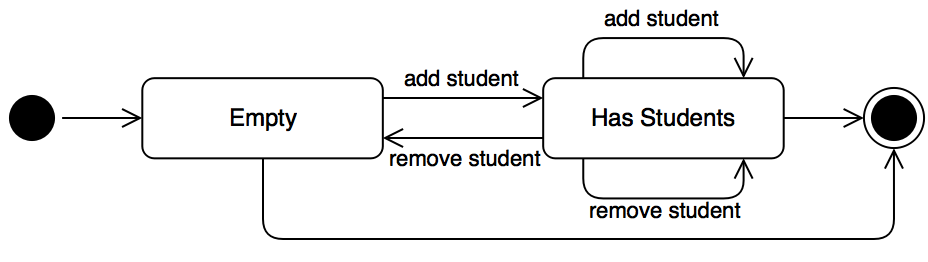
\includegraphics[scale=0.3]{imgs/state/project-enrollment.png}
	\caption[\smref{project-student-enrollment} - State Machine for Project Student Enrollment]{State Machine for Project Student Enrollment (\smref{project-student-enrollment})}
	\figurelabel{sm-project-student-enrollment}
\end{figure}

\noindent The following diagram, \figureref{sm-project-name}, represents a state machine for the Project object. Shown here is the different states involved in the setting of a Project's name.

\begin{figure}[H]
    \smlabel{project-name}
	\centering{}
	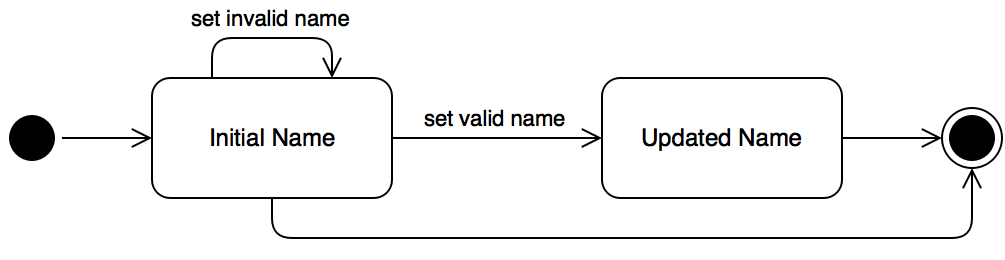
\includegraphics[scale=0.3]{imgs/state/project-name.png}
	\caption[\smref{project-name} - State Machine for Project Name]{State Machine for Project Name (\smref{project-name})}
	\figurelabel{sm-project-name}
\end{figure}

\noindent The following diagram, \figureref{sm-project-ppid-results}, represents a state machine for the Project object. Shown here is the different states involved in showing the results of/running the PPID.

\begin{figure}[H]
    \smlabel{project-ppid-results}
	\centering{}
	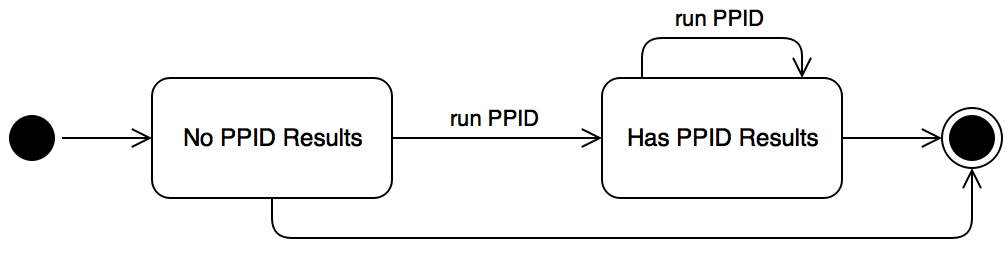
\includegraphics[scale=0.3]{imgs/state/project-ppid-results.png}
	\caption[\smref{project-ppid-results} - State Machine for Project PPID Results]{State Machine for Project PPID Results (\smref{project-ppid-results})}
	\figurelabel{sm-project-ppid-results}
\end{figure}

\subsubsection*{State Machines for Group:}

The following diagram, \figureref{sm-group-enrollment}, represents a state machine for the Group object. Shown here is the different states involved in adding/enrolling students into Groups.

\begin{figure}[H]
    \smlabel{group-enrollment}
	\centering{}
	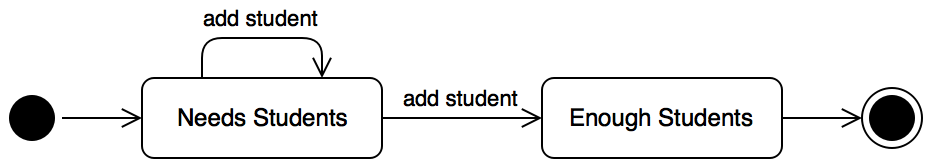
\includegraphics[scale=0.3]{imgs/state/group-enrollment.png}
	\caption[\smref{group-enrollment} - State Machine for Group Enrollment]{State Machine for Group Enrollment (\smref{group-enrollment})}
	\figurelabel{sm-group-enrollment}
\end{figure}

\subsubsection*{State Machines for GroupSize:}

The following diagram, \figureref{sm-group-size-value}, represents a state machine for the GroupSize object. Shown here is the different states involved in updating/setting a new value for the GroupSize.

\begin{figure}[H]
    \smlabel{group-size-value}
	\centering{}
	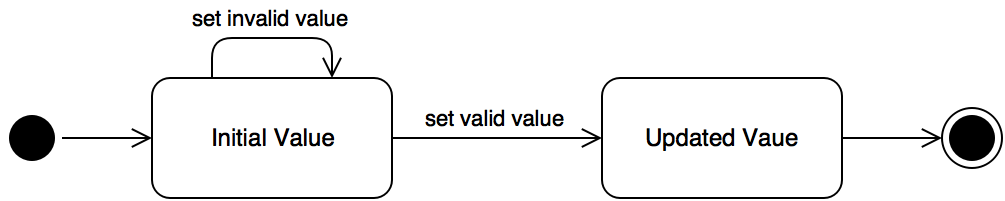
\includegraphics[scale=0.3]{imgs/state/group-size-value.png}
	\caption[\smref{group-size-value} - State Machine for GroupSize Value]{State Machine for GroupSize Value (\smref{group-size-value})}
	\figurelabel{sm-group-size-value}
\end{figure}

\subsubsection*{Sequence Diagrams}

Sequence diagrams are a great visual representation of the many interactions between different objects needed to satisfy one use case. Note that
each object has a vertical dotted line - this represents the time-line of that object. Through the course of the diagram, multiple objects will be created
and destroyed after fulfilling their purpose.

\newpage{}

\subsubsection*{Sequence diagram for ManageEnrollment (\ucref{manage-enrollment}):}

The following figure, \figureref{seq-manage-enrollment}, shows the sequence diagram for the {\it ManageEnrollment} use case. The participating actor for this use case
is the Student user. This figure shows the necessary interactions between the control object, {\it LaunchPPIDControl}, and the entity/boundary objects
in order to manage \ucref{manage-enrollment}.
\begin{figure}[H]
    \seqlabel{manage-enrollment}
	\centering{}
	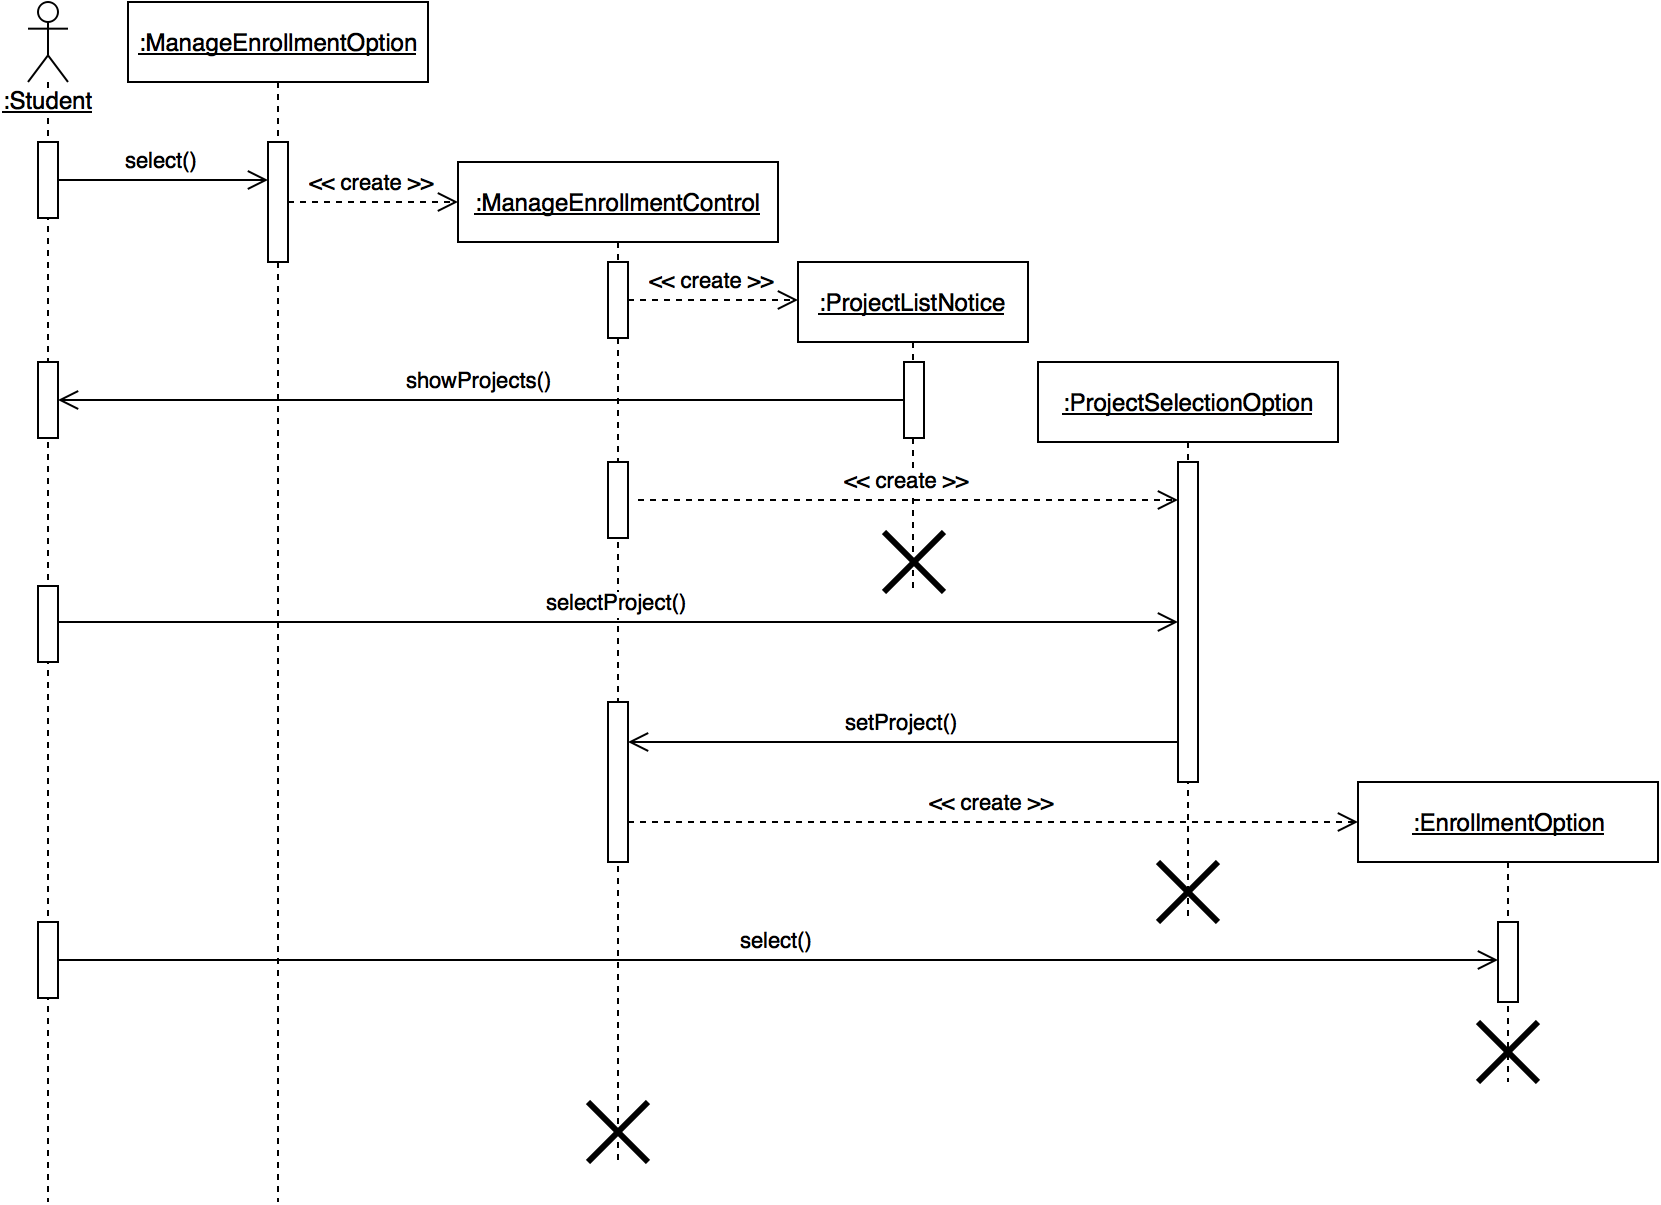
\includegraphics[scale=0.27]{imgs/seq/manage-enrollment.png}
	\caption[\seqref{manage-enrollment} - Sequence Diagram for ManageEnrollment]{Sequence Diagram for ManageEnrollment (\seqref{manage-enrollment})}
	\figurelabel{seq-manage-enrollment}
\end{figure}

\newpage{}

\subsubsection*{Sequence diagram for EditProfile (\ucref{edit-profile}):}

The following figure, {seq-edit-profile}, shows the sequence diagram for the {\it EditProfile} use case. The participating actor is the 
Student user. This figure shows the necessary interactions between the control object, {\it EditProfileControl}, and the entity/boundary objects
in order to manage \ucref{edit-profile}.

\begin{figure}[H]
    \seqlabel{edit-profile}
	\centering{}
	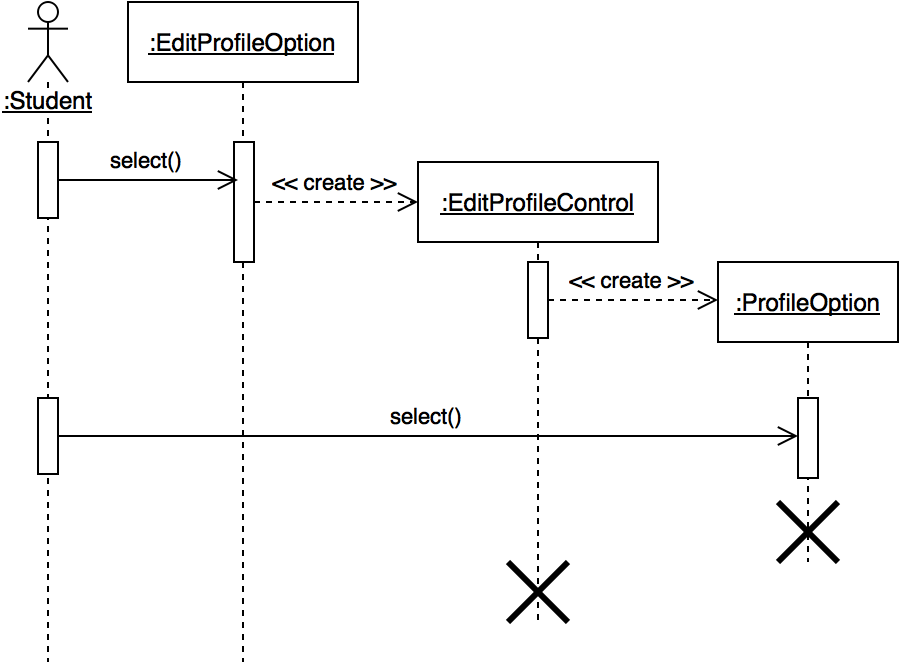
\includegraphics[scale=0.25]{imgs/seq/edit-profile.png}
	\caption[\seqref{edit-profile} - Sequence Diagram for EditProfile]{Sequence Diagram for EditProfile (\seqref{edit-profile})}
	\figurelabel{seq-edit-profile}
\end{figure}

\subsubsection*{Sequence diagram for ManageProject (\ucref{manage-project}):}

The following figure, \figureref{seq-manage-project}, shows the sequence diagram for the {\it ManageProject} use case. The participating actor is the
Student user. This figure shows the necessary interactions between the control object, {\it ManageProjectControl}, and the entity/boundary objects 
in order to manage \ucref{manage-project}.

\begin{figure}[H]
    \seqlabel{manage-project}
	\centering{}
	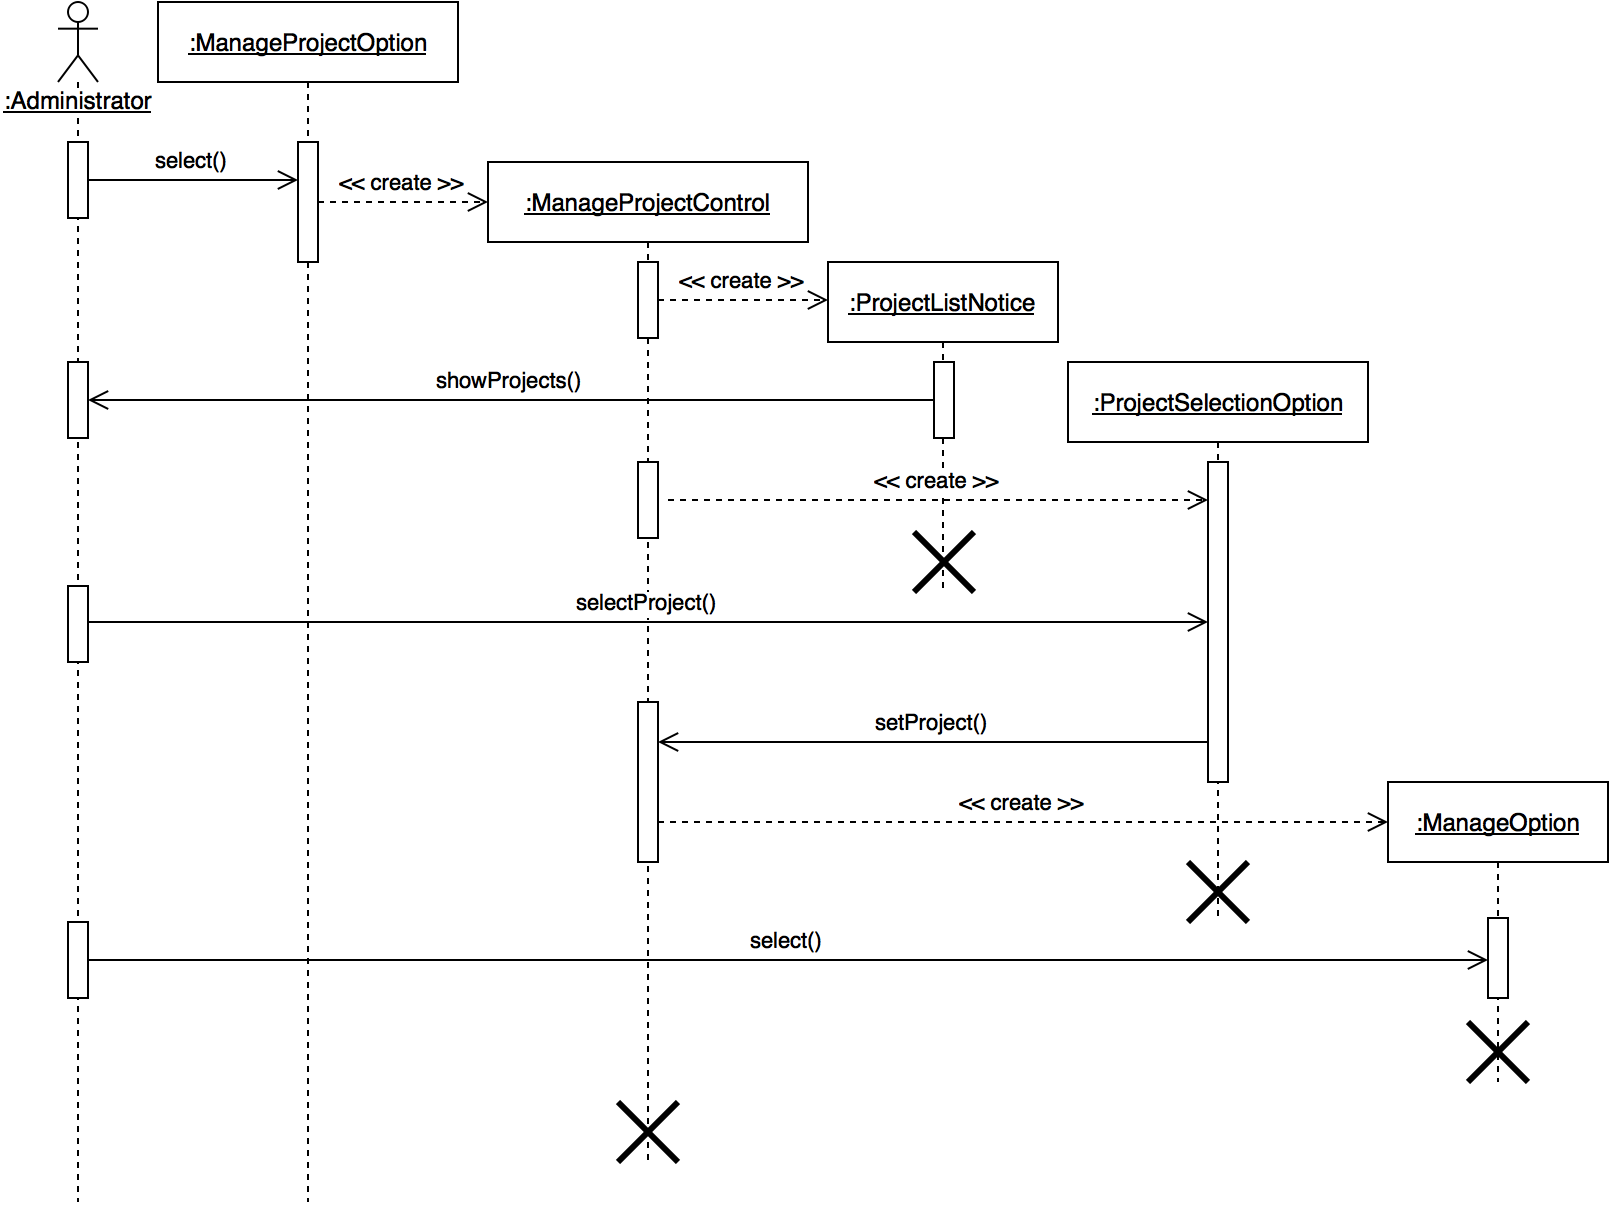
\includegraphics[scale=0.24]{imgs/seq/manage-project.png}
	\caption[\seqref{manage-project} - Sequence Diagram for ManageProject]{Sequence Diagram for ManageProject (\seqref{manage-project})}
	\figurelabel{seq-manage-project}
\end{figure}

\subsubsection*{Sequence diagram for CreateNewProject (\ucref{create-new-project}):}

The following figure, \figureref{seq-create-new-project}, shows the sequence diagram for the {\it CreateNewProject} use case. The participating actor for this use case is
the Administrator user. This figure shows the necessary interactions between the control object, {\it CreateNewProjectControl}, and the
entity/boundary objects in order to manage \ucref{create-new-project}.

\begin{figure}[H]
    \seqlabel{create-new-project}
	\centering{}
	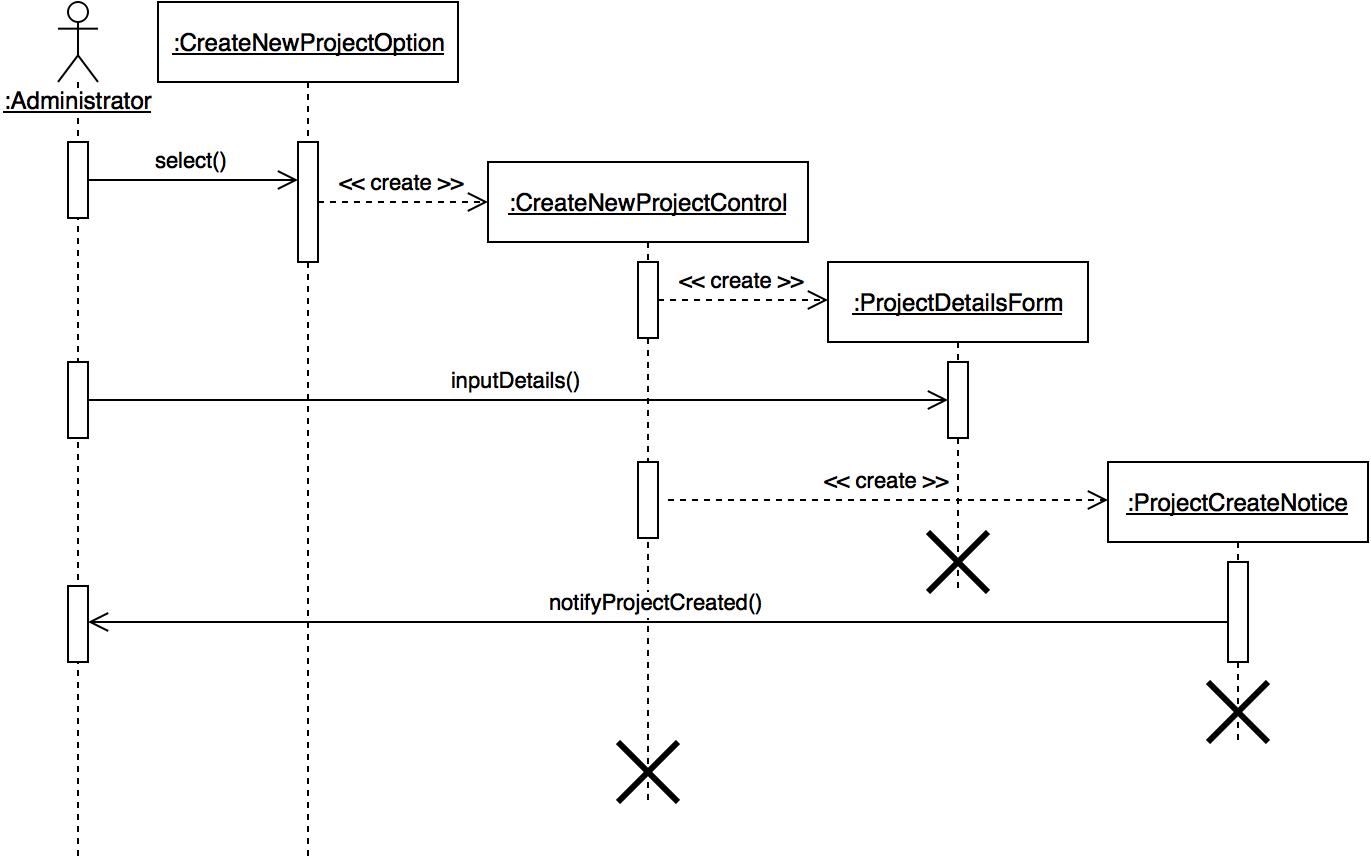
\includegraphics[scale=0.24]{imgs/seq/create-new-project.png}
	\caption[\seqref{create-new-project} - Sequence Diagram for CreateNewProject]{Sequence Diagram for CreateNewProject (\seqref{create-new-project})}
	\figurelabel{seq-create-new-project}
\end{figure}

\subsubsection*{Sequence diagram for LaunchPPID (\ucref{launch-ppid}):}

The following figure, \figureref{seq-launch-ppid}, shows the sequence diagram for the {\it LaunchPPID} use case. The participating actor for this use case is
the Administrator user. This figure shows the necessary interactions between the control object, {\it LaunchPPIDControl}, and the
entity/boundary objects in order to manage \ucref{launch-ppid}.

\begin{figure}[H]
    \seqlabel{launch-ppid}
	\centering{}
	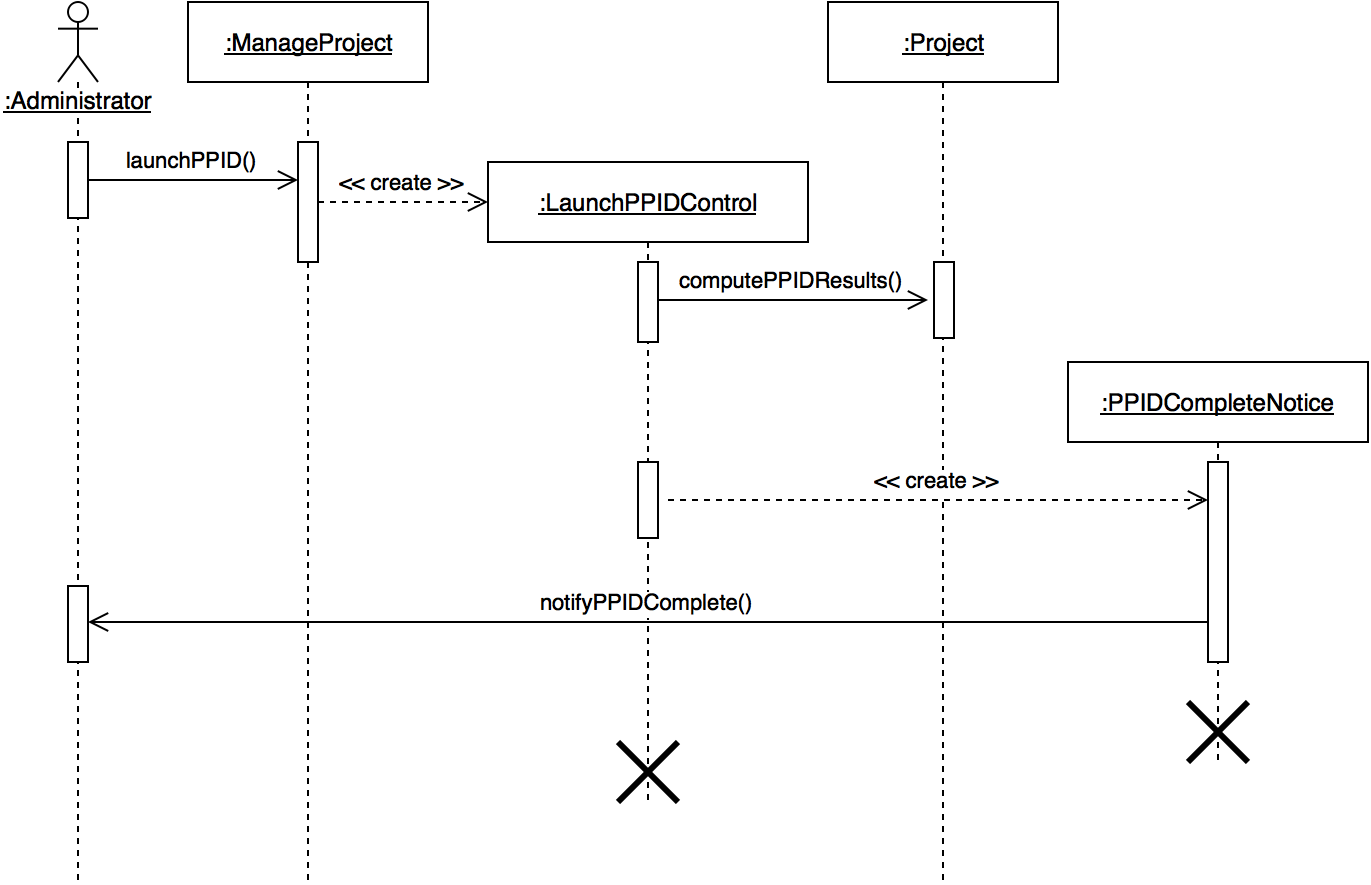
\includegraphics[scale=0.25]{imgs/seq/launch-ppid.png}
	\caption[\seqref{launch-ppid} - Sequence Diagram for LaunchPPID]{Sequence Diagram for LaunchPPID (\seqref{launch-ppid})}
	\figurelabel{seq-launch-ppid}
\end{figure}

\subsubsection*{Sequence diagram for InsufficientStudentsError (\ucref{insufficient-students-error}):}

The following figure, \figureref{seq-insufficient-students-error}, shows the sequence diagram for the {\it InsufficientStudentsError} use case. The participating actor for this use case is
the Administrator user. This figure shows the necessary interactions between the control object, {\it InsufficientStudentsErrorControl}, and the
entity/boundary objects in order to manage \ucref{insufficient-students-error}.

\begin{figure}[H]
    \seqlabel{insufficient-students-error}
	\centering{}
	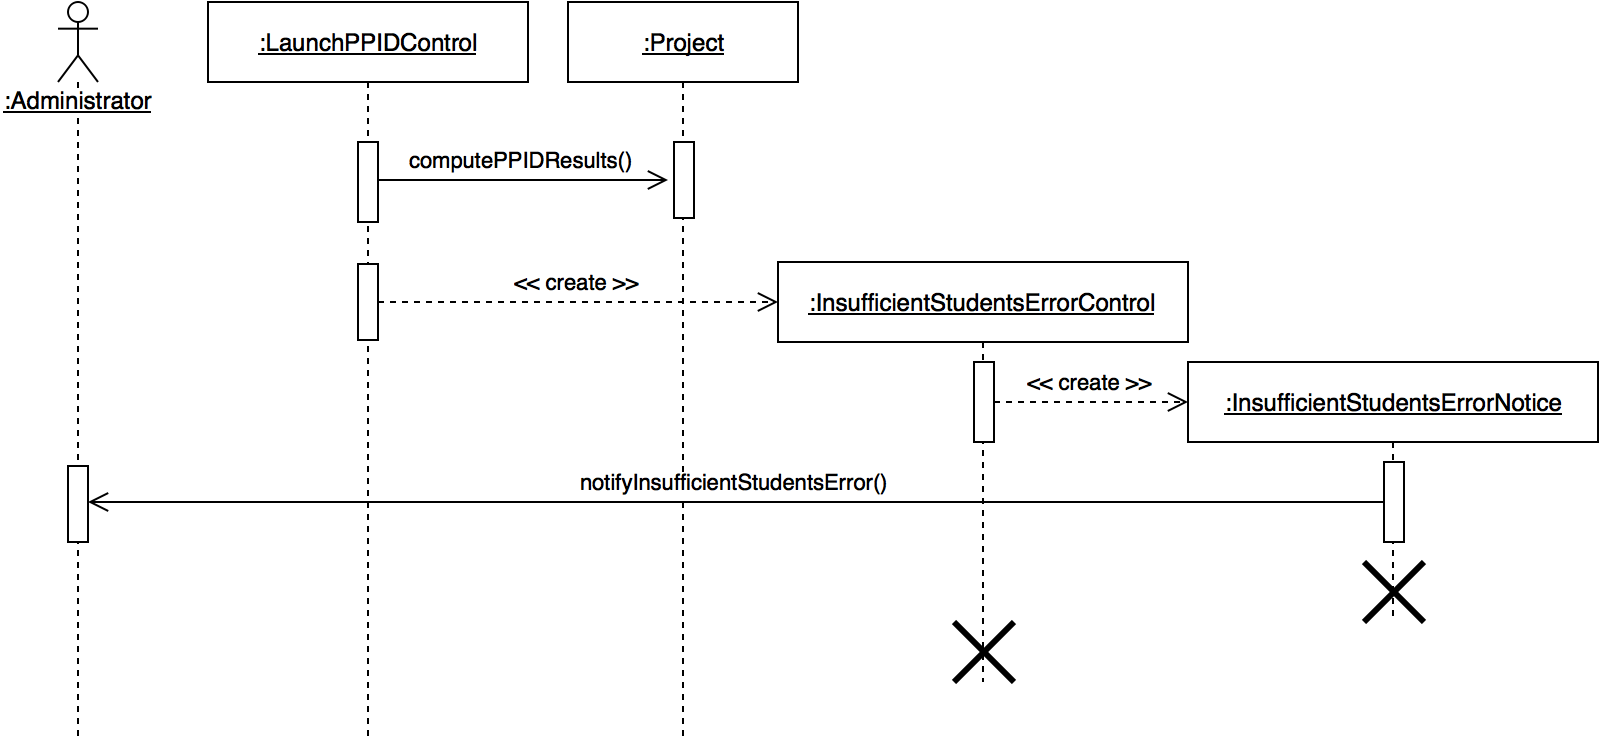
\includegraphics[scale=0.27]{imgs/seq/insufficient-students-error.png}
	\caption[\seqref{insufficient-students-error} - Sequence Diagram for InsufficientStudentsError]{Sequence Diagram for InsufficientStudentsError (\seqref{insufficient-students-error})}
	\figurelabel{seq-insufficient-students-error}
\end{figure}

\subsubsection*{Sequence diagram for ViewPPIDResults (\ucref{view-ppid-results}):}

The following figure, \figureref{seq-view-ppid-results}, shows the sequence diagram for the {\it ViewPPIDResults} use case. The participating actor for this use case is
the Administrator user. This figure shows the necessary interactions between the control object, {\it ViewPPIDResultsControl}, and the
entity/boundary objects in order to manage \ucref{view-ppid-results}.

\begin{figure}[H]
    \seqlabel{view-ppid-results}
	\centering{}
	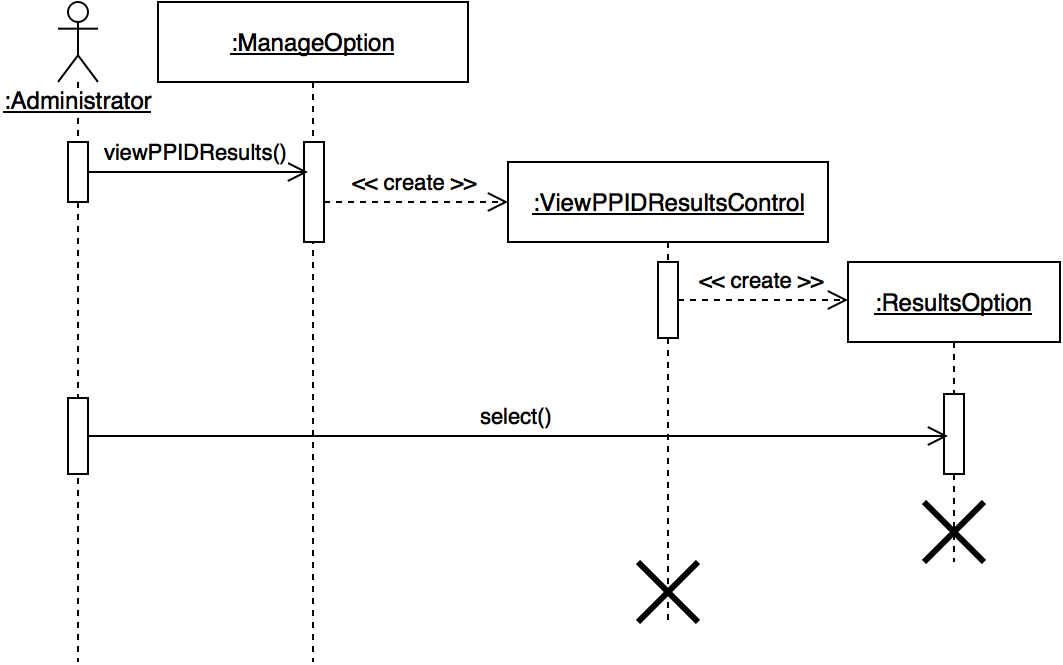
\includegraphics[scale=0.27]{imgs/seq/view-ppid-results.png}
	\caption[\seqref{view-ppid-results} - Sequence Diagram for ViewPPIDResults]{Sequence Diagram for ViewPPIDResults (\seqref{view-ppid-results})}
	\figurelabel{seq-view-ppid-results}
\end{figure}

\newpage{}

\subsubsection*{Sequence diagram for ViewPPIDSummary (\ucref{view-ppid-summary}):}

The following figure, \figureref{seq-view-ppid-summary}, shows the sequence diagram for the {\it ViewPPIDSummary} use case. The participating actor for this use case is
the Administrator user. This figure shows the necessary interactions between the control object, {\it ViewPPIDSummaryControl}, and the
entity/boundary objects in order to manage \ucref{view-ppid-summary}.

\begin{figure}[H]
    \seqlabel{view-ppid-summary}
	\centering{}
	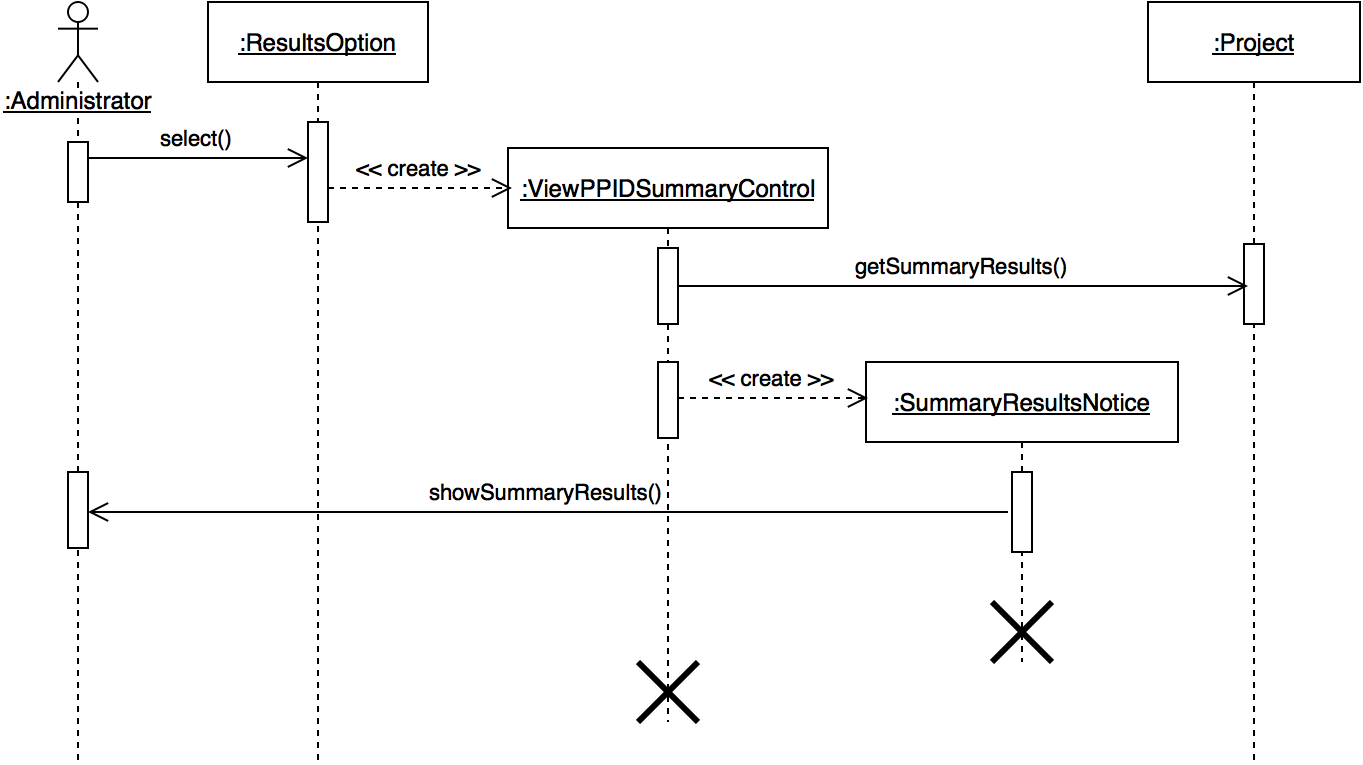
\includegraphics[scale=0.25]{imgs/seq/view-ppid-summary.png}
	\caption[\seqref{view-ppid-summary} - Sequence Diagram for ViewPPIDSummary]{Sequence Diagram for ViewPPIDSummary (\seqref{view-ppid-summary})}
	\figurelabel{seq-view-ppid-summary}
\end{figure}

\subsubsection*{Sequence diagram for ViewPPIDDDetails (\ucref{view-ppid-details}):}

The following figure, \figureref{seq-view-ppid-details}, shows the sequence diagram for the {\it ViewPPIDDetails} use case. The participating actor for this use case is
the Administrator user. This figure shows the necessary interactions between the control object, {\it ViewPPIDDetailsControl}, and the
entity/boundary objects in order to manage \ucref{view-ppid-details}.

\begin{figure}[H]
    \seqlabel{view-ppid-details}
	\centering{}
	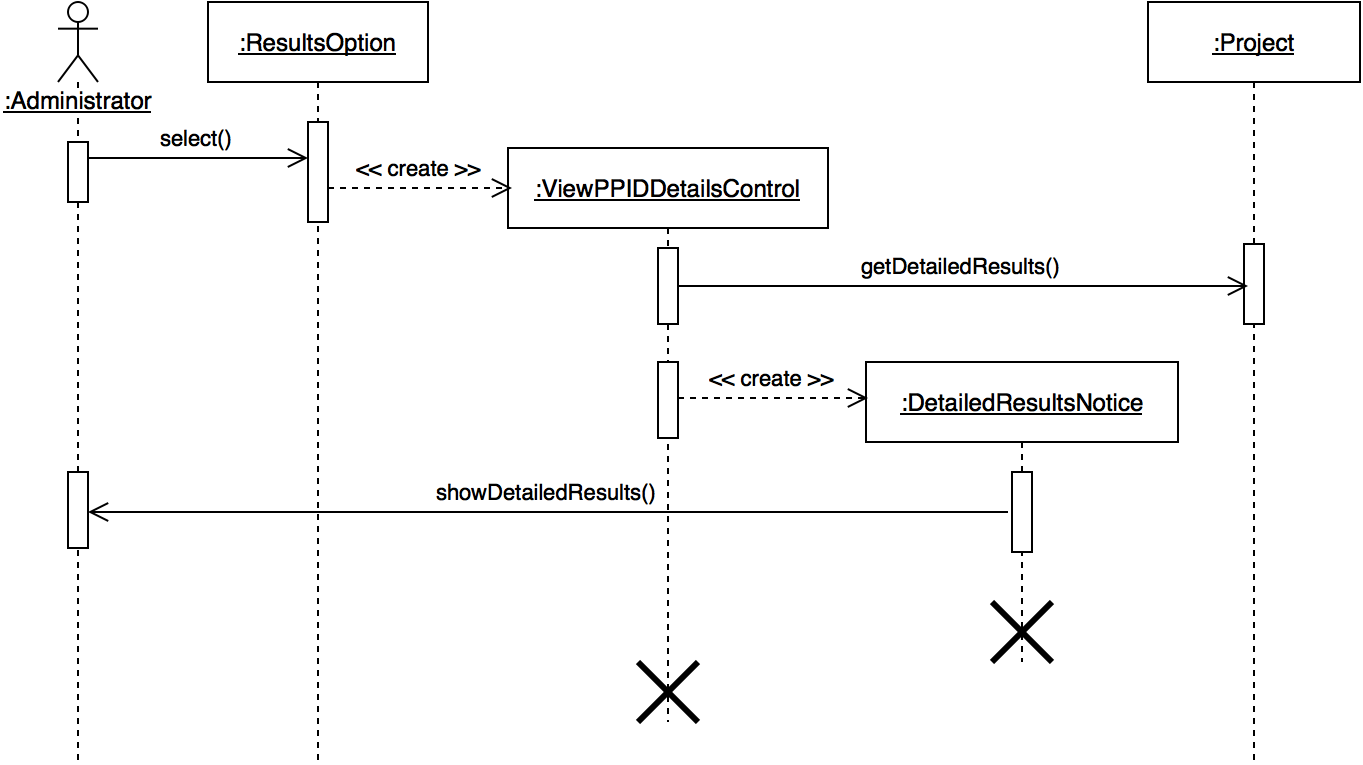
\includegraphics[scale=0.25]{imgs/seq/view-ppid-details.png}
	\caption[\seqref{view-ppid-details} - Sequence Diagram for ViewPPIDDetails]{Sequence Diagram for ViewPPIDDetails (\seqref{view-ppid-details})}
	\figurelabel{seq-view-ppid-details}
\end{figure}

\subsubsection*{Sequence diagram for EditProjectDetails (\ucref{edit-project-details}):}

The following figure, \figureref{seq-edit-project-details}, shows the sequence diagram for the {\it EditProjectDetails} use case. The participating actor for this use case is
the Administrator user. This figure shows the necessary interactions between the control object, {\it EditProjectDetailsControl}, and the
entity/boundary objects in order to manage \ucref{edit-project-details}.

\begin{figure}[H]
    \seqlabel{edit-project-details}
	\centering{}
	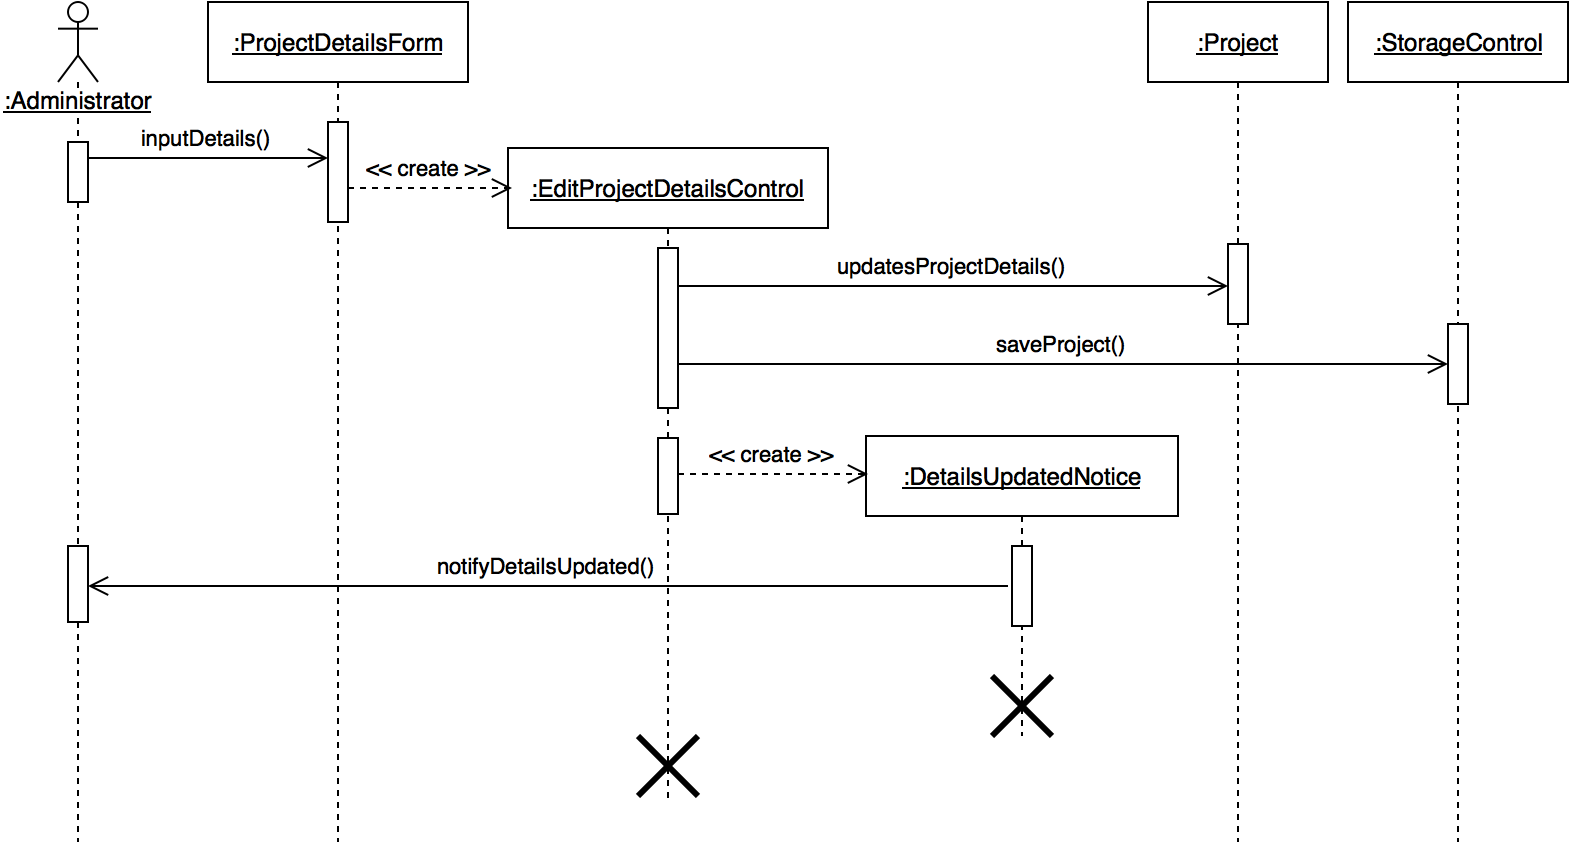
\includegraphics[scale=0.25]{imgs/seq/edit-project-details.png}
	\caption[\seqref{edit-project-details} - Sequence Diagram for EditProjectDetails]{Sequence Diagram for EditProjectDetails (\seqref{edit-project-details})}
	\figurelabel{seq-edit-project-details}
\end{figure}

\subsubsection*{Sequence diagram for EditProject (\ucref{edit-project}):}

The following figure, \figureref{seq-edit-project}, shows the sequence diagram for the {\it EditProject} use case. The participating actor for this use case is
the Administrator user. This figure shows the necessary interactions between the control object, {\it EditProjectControl}, and the
entity/boundary objects in order to manage \ucref{edit-project}.

\begin{figure}[H]
    \seqlabel{edit-project}
	\centering{}
	\includegraphics[scale=0.25]{imgs/seq/edit-project.png}
	\caption[\seqref{edit-project} - Sequence Diagram for EditProject]{Sequence Diagram for EditProject (\seqref{edit-project})}
	\figurelabel{seq-edit-project}
\end{figure}

\subsubsection*{Sequence diagram for JoinProject (\ucref{join-project})}

The following figure, \figureref{seq-join-project}, shows the sequence diagram for the {\it JoinProject} use case. The participating actor for this use case is
the Student user. This figure shows the necessary interactions between the control object, {\it JoinProjectControl}, and the
entity/boundary objects in order to manage \ucref{join-project}.

\begin{figure}[H]
    \seqlabel{join-project}
	\centering{}
	\includegraphics[scale=0.25]{imgs/seq/join-project.png}
	\caption[\seqref{join-project} - Sequence Diagram for JoinProject]{Sequence Diagram for JoinProject (\seqref{join-project})}
	\figurelabel{seq-join-project}
\end{figure}

\subsubsection*{Sequence diagram for LeaveProject (\ucref{leave-project})}

The following figure, \figureref{seq-leave-project}, shows the sequence diagram for the {\it LeaveProject} use case. The participating actor for this use case is
the Student user. This figure shows the necessary interactions between the control object, {\it LeaveProjectControl}, and the
entity/boundary objects in order to manage \ucref{leave-project}.

\begin{figure}[H]
    \seqlabel{leave-project}
	\centering{}
	\includegraphics[scale=0.25]{imgs/seq/leave-project.png}
	\caption[\seqref{leave-project} - Sequence Diagram for LeaveProject]{Sequence Diagram for LeaveProject (\seqref{leave-project})}
	\figurelabel{seq-leave-project}
\end{figure}

\subsubsection*{Sequence diagram for EditPersonalValues (\ucref{edit-personal-values})}

The following figure, \figureref{seq-edit-personal-values}, shows the sequence diagram for the {\it EditPersonalValues} use case. The participating actor for this use case is
the Student user. This figure shows the necessary interactions between the control object, {\it EditPersonalValuesControl}, and the
entity/boundary objects in order to manage \ucref{edit-personal-values}.

\begin{figure}[H]
    \seqlabel{edit-personal-values}
	\centering{}
	\includegraphics[scale=0.25]{imgs/seq/edit-personal-values.png}
	\caption[\seqref{edit-personal-values} - Sequence Diagram for EditPersonalValues]{Sequence Diagram for EditPersonalValues (\seqref{edit-personal-values})}
	\figurelabel{seq-edit-personal-values}
\end{figure}

\subsubsection*{Sequence diagram for EditDesiredValues (\ucref{edit-desired-values})}

The following figure, \figureref{seq-edit-desired-values}, shows the sequence diagram for the {\it EditDesiredValues} use case. The participating actor for this use case is
the Student user. This figure shows the necessary interactions between the control object, {\it EditDesiredValuesControl}, and the
entity/boundary objects in order to manage \ucref{edit-desired-values}.

\begin{figure}[H]
    \seqlabel{edit-desired-values}
	\centering{}
	\includegraphics[scale=0.25]{imgs/seq/edit-desired-values.png}
	\caption[\seqref{edit-desired-values} - Sequence Diagram for EditDesiredValues]{Sequence Diagram for EditDesiredValues (\seqref{edit-desired-values})}
	\figurelabel{seq-edit-desired-values}
\end{figure}

\subsubsection*{Sequence diagram for InvalidInputError (\ucref{invalid-input-error})}

The following figure, \figureref{seq-invalid-input-error}, shows the sequence diagram for the {\it InvalidInputError} use case. The participating actor for this use case is
the Administrator user. This figure shows the necessary interactions between the control object, {\it InvalidInputErrorControl}, and the
entity/boundary objects in order to manage \ucref{invalid-input-error}.

\begin{figure}[H]
    \seqlabel{invalid-input-error}
	\centering{}
	\includegraphics[scale=0.27]{imgs/seq/invalid-input-error.png}
	\caption[\seqref{invalid-input-error} - Sequence Diagram for InvalidInputError]{Sequence Diagram for InvalidInputError (\seqref{invalid-input-error})}
	\figurelabel{seq-invalid-input-error}
\end{figure}

\subsubsection*{Sequence diagram for EditProjectName (\ucref{edit-project-name})}

The following figure, \figureref{seq-edit-project-name}, shows the sequence diagram for the {\it EditProjectName} use case. The participating actor for this use case is the Administrator user. This figure shows the necessary interactions between the control object, {\it EditProjectNameControl}, and the
entity/boundary objects in order to manage \ucref{edit-project-name}.

\begin{figure}[H]
    \seqlabel{edit-project-name}
	\centering{}
	\includegraphics[scale=0.27]{imgs/seq/edit-project-name.png}
	\caption[\seqref{edit-project-name} - Sequence Diagram for EditProjectName]{Sequence Diagram for EditProjectName (\seqref{edit-project-name})}
	\figurelabel{seq-edit-project-name}
\end{figure}

\newpage{}

\subsubsection*{Sequence diagram for ProjectExistsError (\ucref{project-exists-error})}

The following figure, \figureref{seq-project-exists-error}, shows the sequence diagram for the {\it ProjectExistsError} use case. The participating actor for this use case is
the Administrator user. This figure shows the necessary interactions between the control object, {\it ProjectExistsErorrControl}, and the
entity/boundary objects in order to manage \ucref{project-exists-error}.

\begin{figure}[H]
    \seqlabel{project-exists-error}
	\centering{}
	\includegraphics[scale=0.25]{imgs/seq/project-exists-error.png}
	\caption[\seqref{project-exists-error} - Sequence Diagram for ProjectExistsError]{Sequence Diagram for ProjectExistsError (\seqref{project-exists-error})}
	\figurelabel{seq-project-exists-error}
\end{figure}

\subsubsection*{Sequence diagram for EditGroupSize (\ucref{edit-group-size})}

The following figure, \figureref{seq-edit-group-size}, shows the sequence diagram for the {\it EditGroupSize} use case. The participating actor for this use case is
the Administrator user. This figure shows the necessary interactions between the control object, {\it EditGroupSizeControl}, and the
entity/boundary objects in order to manage \ucref{edit-group-size}.

\begin{figure}[H]
    \seqlabel{edit-group-size}
	\centering{}
	\includegraphics[scale=0.27]{imgs/seq/edit-group-size.png}
	\caption[\seqref{edit-group-size} - Sequence Diagram for EditGroupSize]{Sequence Diagram for EditGroupSize (\seqref{edit-group-size})}
	\figurelabel{seq-edit-group-size}
\end{figure}

\subsubsection*{Sequence diagram for InvalidGroupSizeError (\ucref{invalid-group-size-error})}

The following figure, \figureref{seq-invalid-group-size-error}, shows the sequence diagram for the {\it InvalidGroupSizeError} use case. The participating actor for this use case is
the Administrator user. This figure shows the necessary interactions between the control object, {\it InvalidGroupSizeErrorControl}, and the
entity/boundary objects in order to manage \ucref{invalid-group-size-error}.

\begin{figure}[H]
    \seqlabel{invalid-group-size-error}
	\centering{}
	\includegraphics[scale=0.27]{imgs/seq/invalid-group-size-error.png}
	\caption[\seqref{invalid-group-size-error} - Sequence Diagram for InvalidGroupSizeError]{Sequence Diagram for InvalidGroupSizeError (\seqref{invalid-group-size-error})}
	\figurelabel{seq-invalid-group-size-error}
\end{figure}

\subsubsection*{Sequence diagram for StorageError (\ucref{storage-error})}

The following figure, \figureref{seq-storage-error}, shows the sequence diagram for the {\it StorageError} use case. The participating actor for this use case is
the User (both Administrator and Student). This figure shows the necessary interactions between the control object, {\it StorageErrorControl}, and the
entity/boundary objects in order to manage \ucref{storage-error}.

\begin{figure}[H]
    \seqlabel{storage-error}
	\centering{}
	\includegraphics[scale=0.27]{imgs/seq/storage-error.png}
	\caption[\seqref{storage-error} - Sequence Diagram for StorageError]{Sequence Diagram for StorageError (\seqref{storage-error})}
	\figurelabel{seq-storage-error}
\end{figure}

\newpage{}

\subsubsection*{Sequence diagram for StorageReadError (\ucref{storage-read-error})}

The following figure, \figureref{seq-storage-read-error}, shows the sequence diagram for the {\it StorageReadError} use case. The participating actor for this use case is
the User (both Administrator and Student). This figure shows the necessary interactions between the control object, {\it StorageReadErrorControl}, and the
entity/boundary objects in order to manage \ucref{storage-read-error}.

\begin{figure}[H]
    \seqlabel{storage-read-error}
	\centering{}
	\includegraphics[scale=0.27]{imgs/seq/storage-read-error.png}
	\caption[\seqref{storage-read-error} - Sequence Diagram for StorageReadError]{Sequence Diagram for StorageReadError (\seqref{storage-read-error})}
	\figurelabel{seq-storage-read-error}
\end{figure}

\subsubsection*{Sequence diagram for StorageOpenError (\ucref{storage-open-error})}

The following figure, \figureref{seq-storage-open-error}, shows the sequence diagram for the {\it StorageOpenError} use case. The participating actor for this use case is
the User (both Administrator and Student). This figure shows the necessary interactions between the control object, {\it StorageOpenErrorControl}, and the
entity/boundary objects in order to manage \ucref{storage-open-error}.

\begin{figure}[H]
    \seqlabel{storage-open-error}
	\centering{}
	\includegraphics[scale=0.27]{imgs/seq/storage-open-error.png}
	\caption[\seqref{storage-open-error} - Sequence Diagram for StorageOpenError]{Sequence Diagram for StorageOpenError (\seqref{storage-open-error})}
	\figurelabel{seq-storage-open-error}
\end{figure}

\newpage{}

\subsubsection*{Sequence diagram for StorageWriteError (\ucref{storage-write-error})}

The following figure, \figureref{seq-storage-write-error}, shows the sequence diagram for the {\it StorageWriteError} use case. The participating actor for this use case is
the User (both Administrator and Student). This figure shows the necessary interactions between the control object, {\it StorageWriteError}, and the
entity/boundary objects in order to manage \ucref{storage-write-error}.

\begin{figure}[H]
    \seqlabel{storage-write-error}
	\centering{}
	\includegraphics[scale=0.27]{imgs/seq/storage-write-error.png}
	\caption[\seqref{storage-write-error} - Sequence Diagram for StorageWriteError]{Sequence Diagram for StorageWriteError (\seqref{storage-write-error})}
	\figurelabel{seq-storage-write-error}
\end{figure}

\end{document}
